To make maximal use of the event information we have performed a multivariate analysis 
using a multivariate classifier based on the Boosted Decision Tree (BDT) technique. 
The BDT is implemented using the TMVA~\cite{tmva} toolkit and has been 
successfully applied in high energy physics to increase the 
statistical significance of a signal extraction
It requires less training than other multivariate classifiers and 
it is insensitive to the inclusion of poorly discriminating input variables.

In addition to the $\WW$ preselection, we apply a loose cut on the
maximum $\mll$ to enhance the signal-to-background ratio shown in Table~\ref{tab:presel_tmva_analysis}. 
In addition to the selection variables for the cut-based analysis, the multivariate signal extraction 
procedure uses the following ones: 
\begin{itemize}
\item $\Delta R_{\Lep\Lep}\equiv\sqrt{\deletall^2 + \delphill^2}$ between the leptons, 
with $\deletall$ the $\eta$ difference between the leptons, 
which has similar properties as $\delphill$
\item lepton flavors ($\mu\mu$, $ee$, $e\mu$ or $\mu e$ );
\item finally, for the 1-jet bin, the azimutal angles between the dilepton 
system and $\met$, and between the dilepton system and the 
highest $\pt$ jet, are included.
\end{itemize}

The distributions for SM Higgs signal and background for all the variables used in the 
multivariate analysis for a Higgs mass of 160 $\GeV$ are shown in Appendix~\ref{app:mvaplots}. 
The training has been carried out separately in the 0-jet and 1-jet bins 
for different Higgs masses using the corresponding signal samples. For the background, 
we have considered $\WW$ processes only for now.  The classifier outputs 
for different Higgs masses and splitting in jet bins and flavor final states are shown in 
Figures~\ref{fig:histo_mva_130} to~\ref{fig:histo_mva_200}.
This analysis technique is not performed 
in the 2-jet bin case due to the limited amount of simulated events for the main background samples.

We follow two approaches for the MVA analysis: either a cut on the MVA output or use of the 
full shape of the classifier output. The cut on the MVA output has been chosen to 
obtain roughly the same background component, which yields in about 10-15\% higher signal 
efficiency. 
The expected number of signal and background events for an integrated luminosity 
of 1 $\ifb$, after applying the full multivariate analysis selection in the 0-jet and 1-jet 
bin cases are listed in Tables~\ref{tab:mvasel0j} and ~\ref{tab:mvasel1j}, respectively. 
The $gg \to H \to WW$ simulated events are reweighted to match the Higgs $\pt$ at NNLO, 
as explained in Section~\ref{sec:datasets}; all data-driven corrections are not applied.

\begin{table}
\begin{center}
\begin{tabular}{|r|c|c|c|c|c|c|c|c|c|c|c|c|}
\hline
$\mHi~~~~~[\GeV]$   & 120 & 130 & 140 & 150 & 160 & 170 & 180 & 190 & 200 & 210 \\
\hline
$\mll<~~~[\GeV]$    &  70 &  80 &  90 & 100 & 100 & 100 & 110 & 120 & 130 & 140 \\
\hline
\end{tabular}
%\vspace{0.5cm}
\begin{tabular}{|r|c|c|c|c|c|c|c|c|c|c|c|}
\hline
$\mHi~~~~~[\GeV]$    & 220 & 230 & 250 & 300 & 350 & 400 & 450 & 500 & 550 & 600 \\
\hline
$\mll<~~~[\GeV]$     & 150 & 230 & 250 & 300 & 350 & 400 & 450 & 500 & 550 & 600 \\
\hline
\end{tabular}
\caption{$\mll$ upper limit requirement as a function of the Higgs mass used to 
enrich the background datasets of signal-like events. These samples are employed 
in the training of the multivariate classifier used for the signal 
extraction.\label{tab:presel_tmva_analysis}}
\end{center}
\end{table}

\begin{figure}[!ht]
\begin{center}
   \subfigure[]{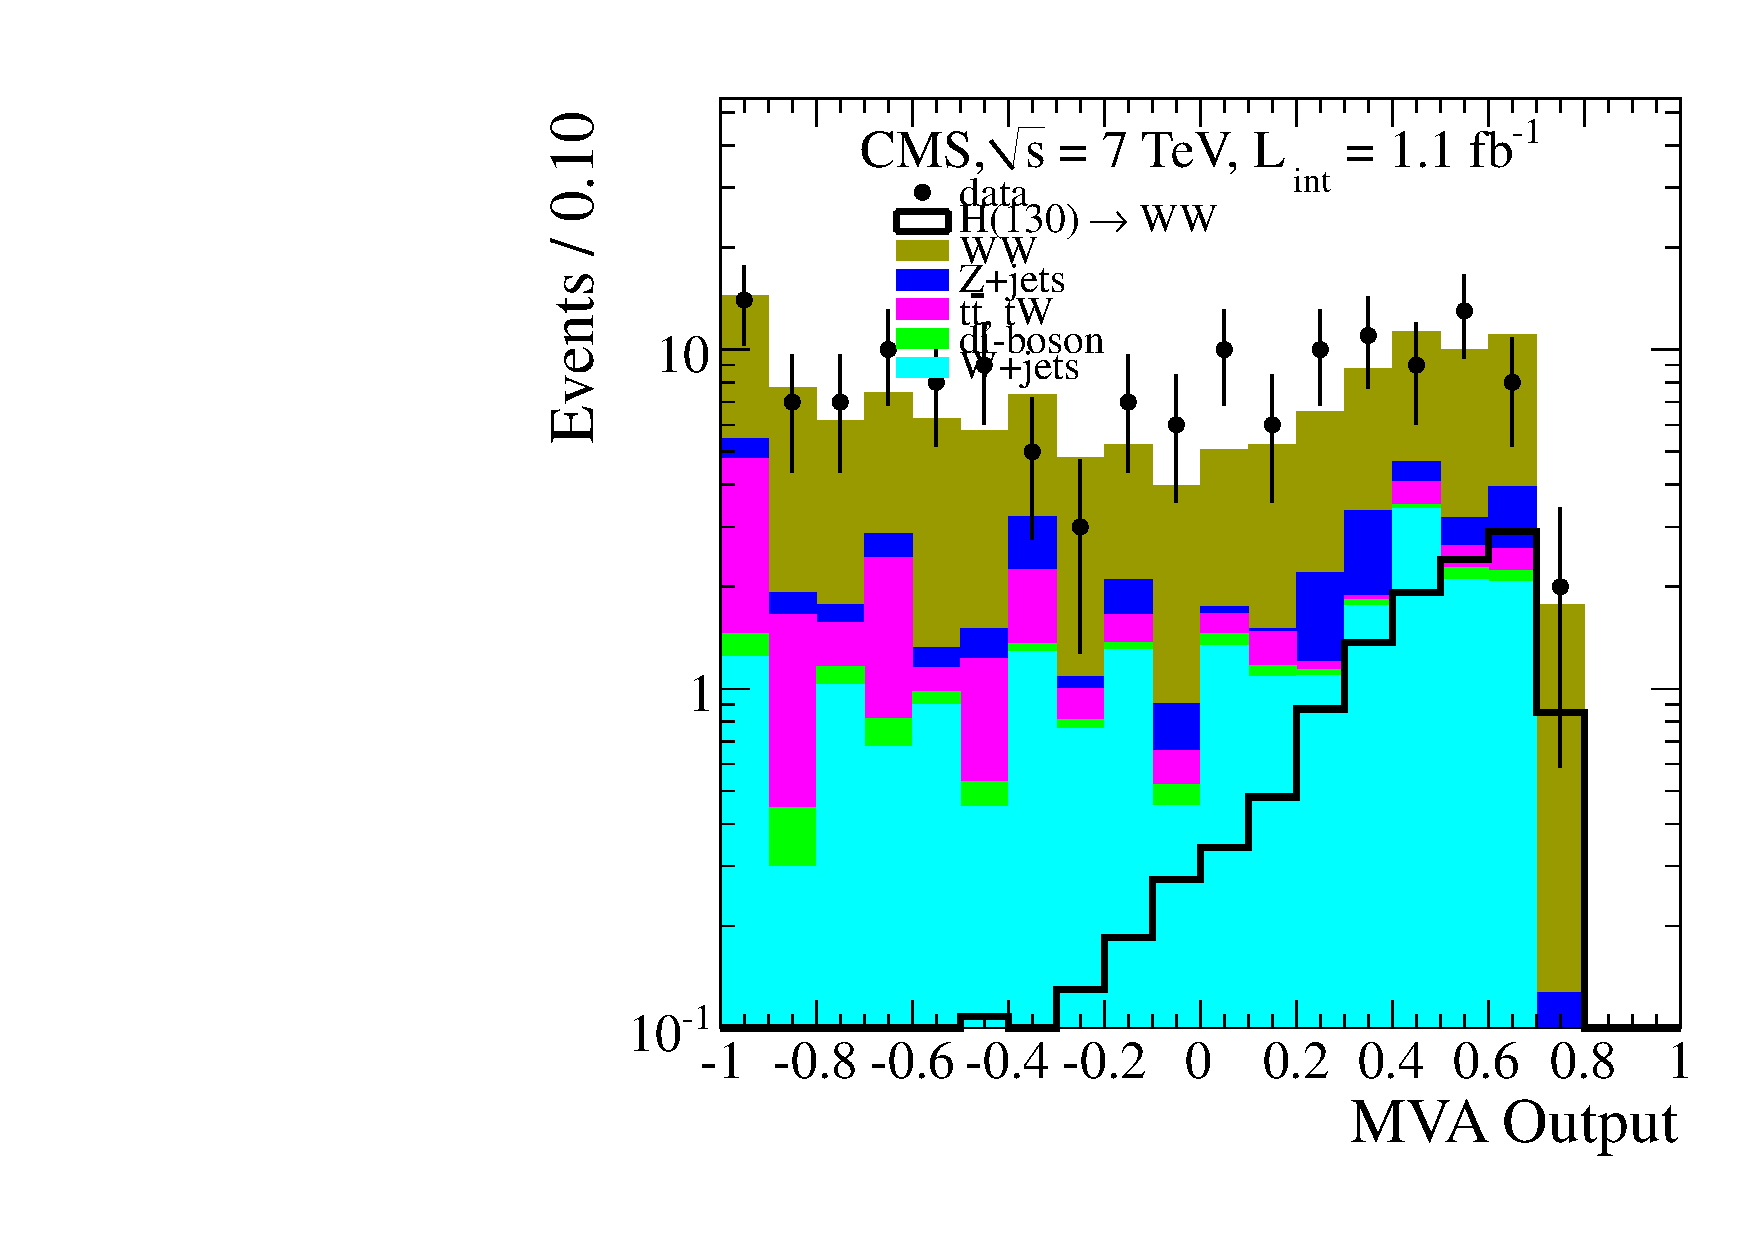
\includegraphics[width=0.49\textwidth,angle=0]{figures/histo_mva_130_0j_sf.pdf}} 
   \subfigure[]{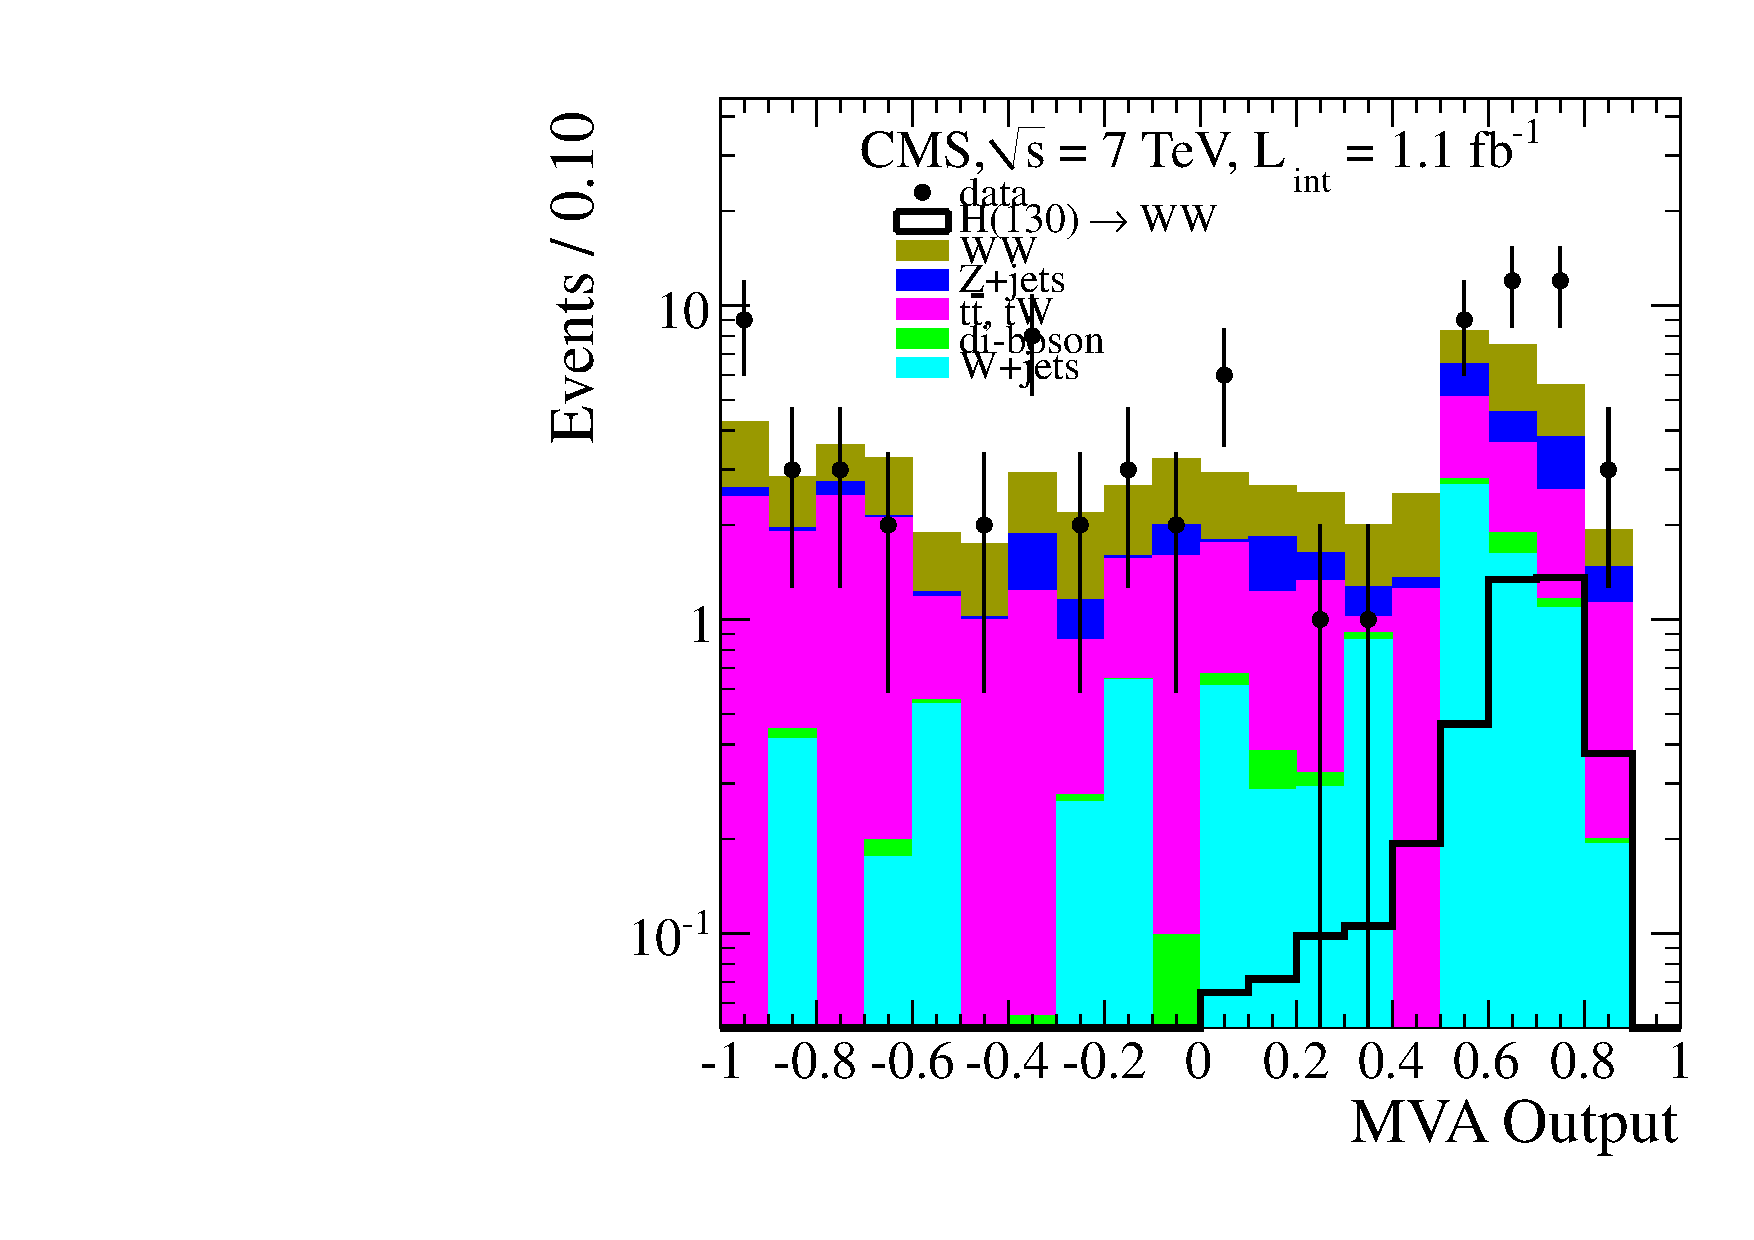
\includegraphics[width=0.49\textwidth,angle=0]{figures/histo_mva_130_1j_sf.pdf}} \\ 
   \subfigure[]{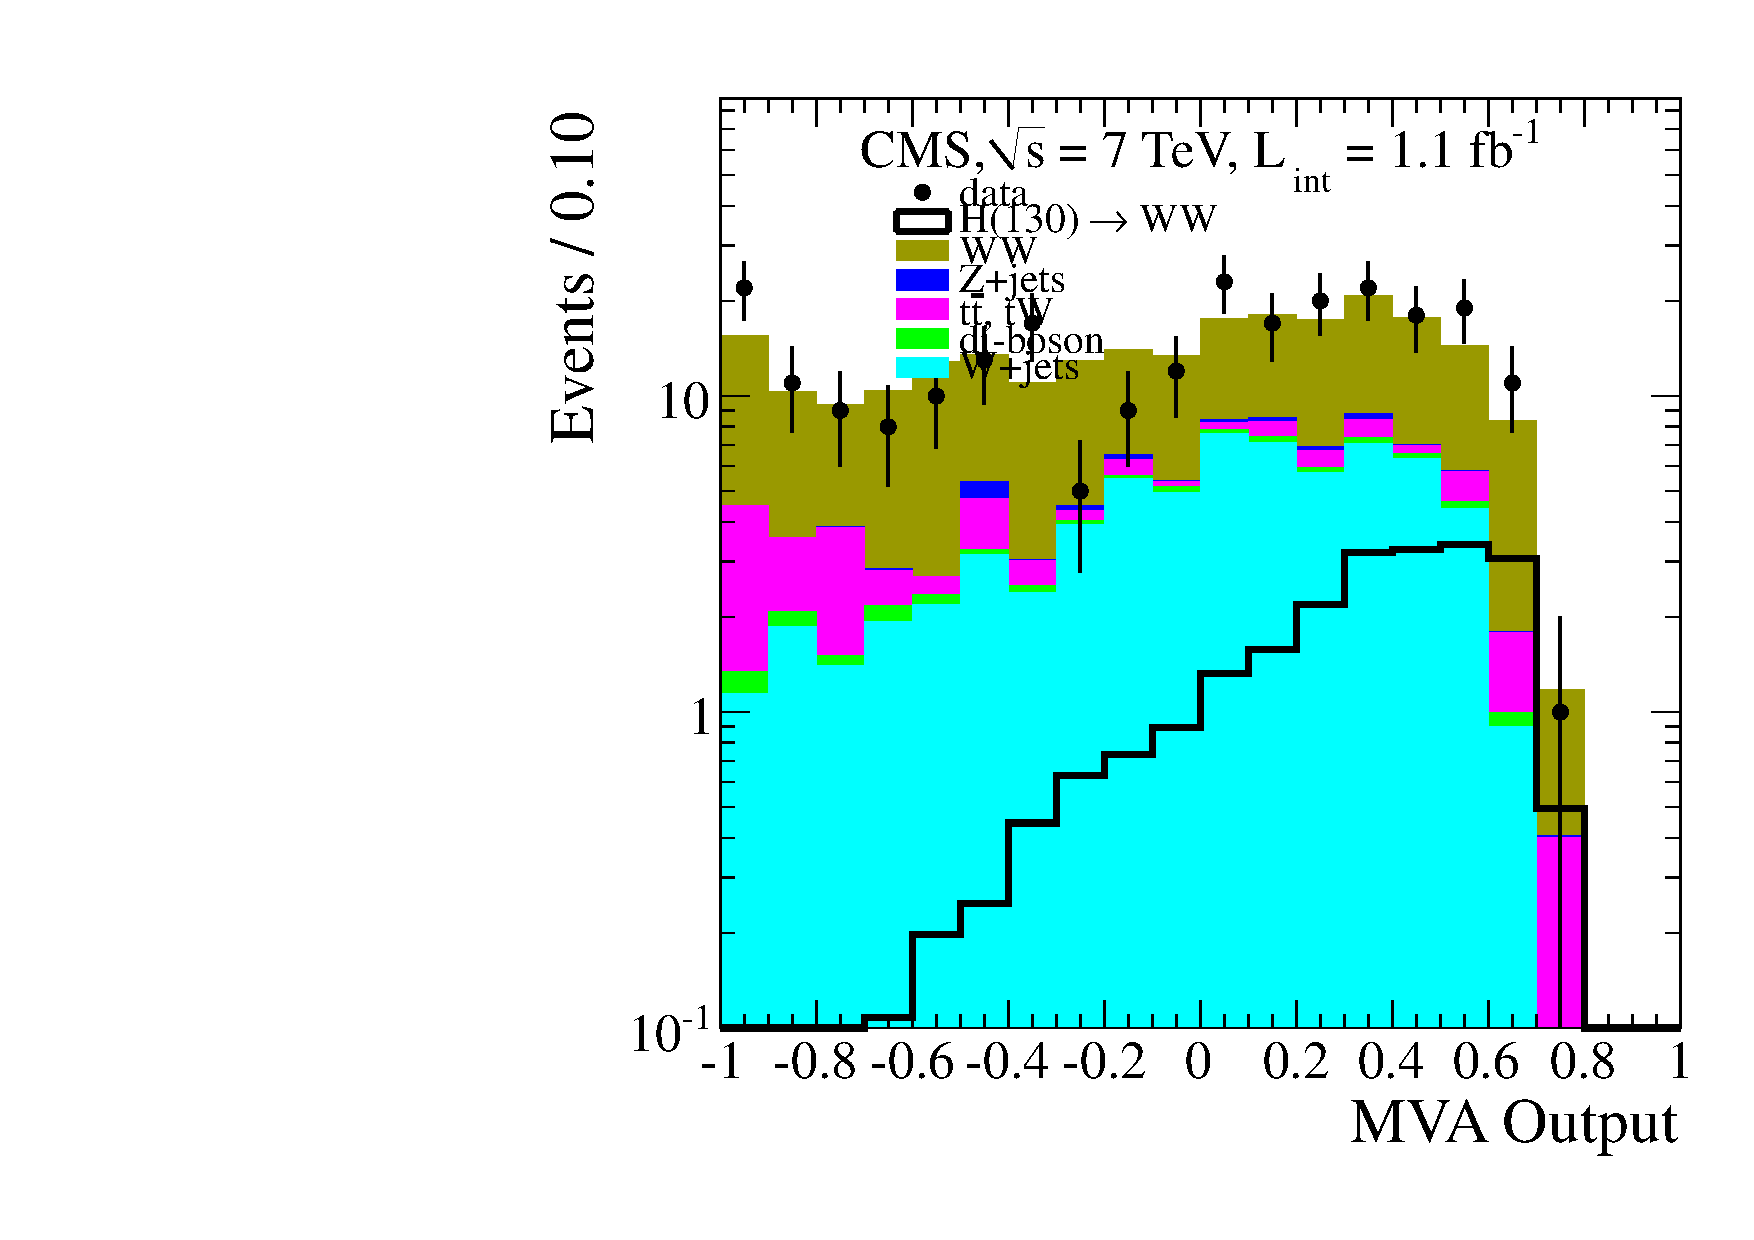
\includegraphics[width=0.49\textwidth,angle=0]{figures/histo_mva_130_0j_of.pdf}} 
   \subfigure[]{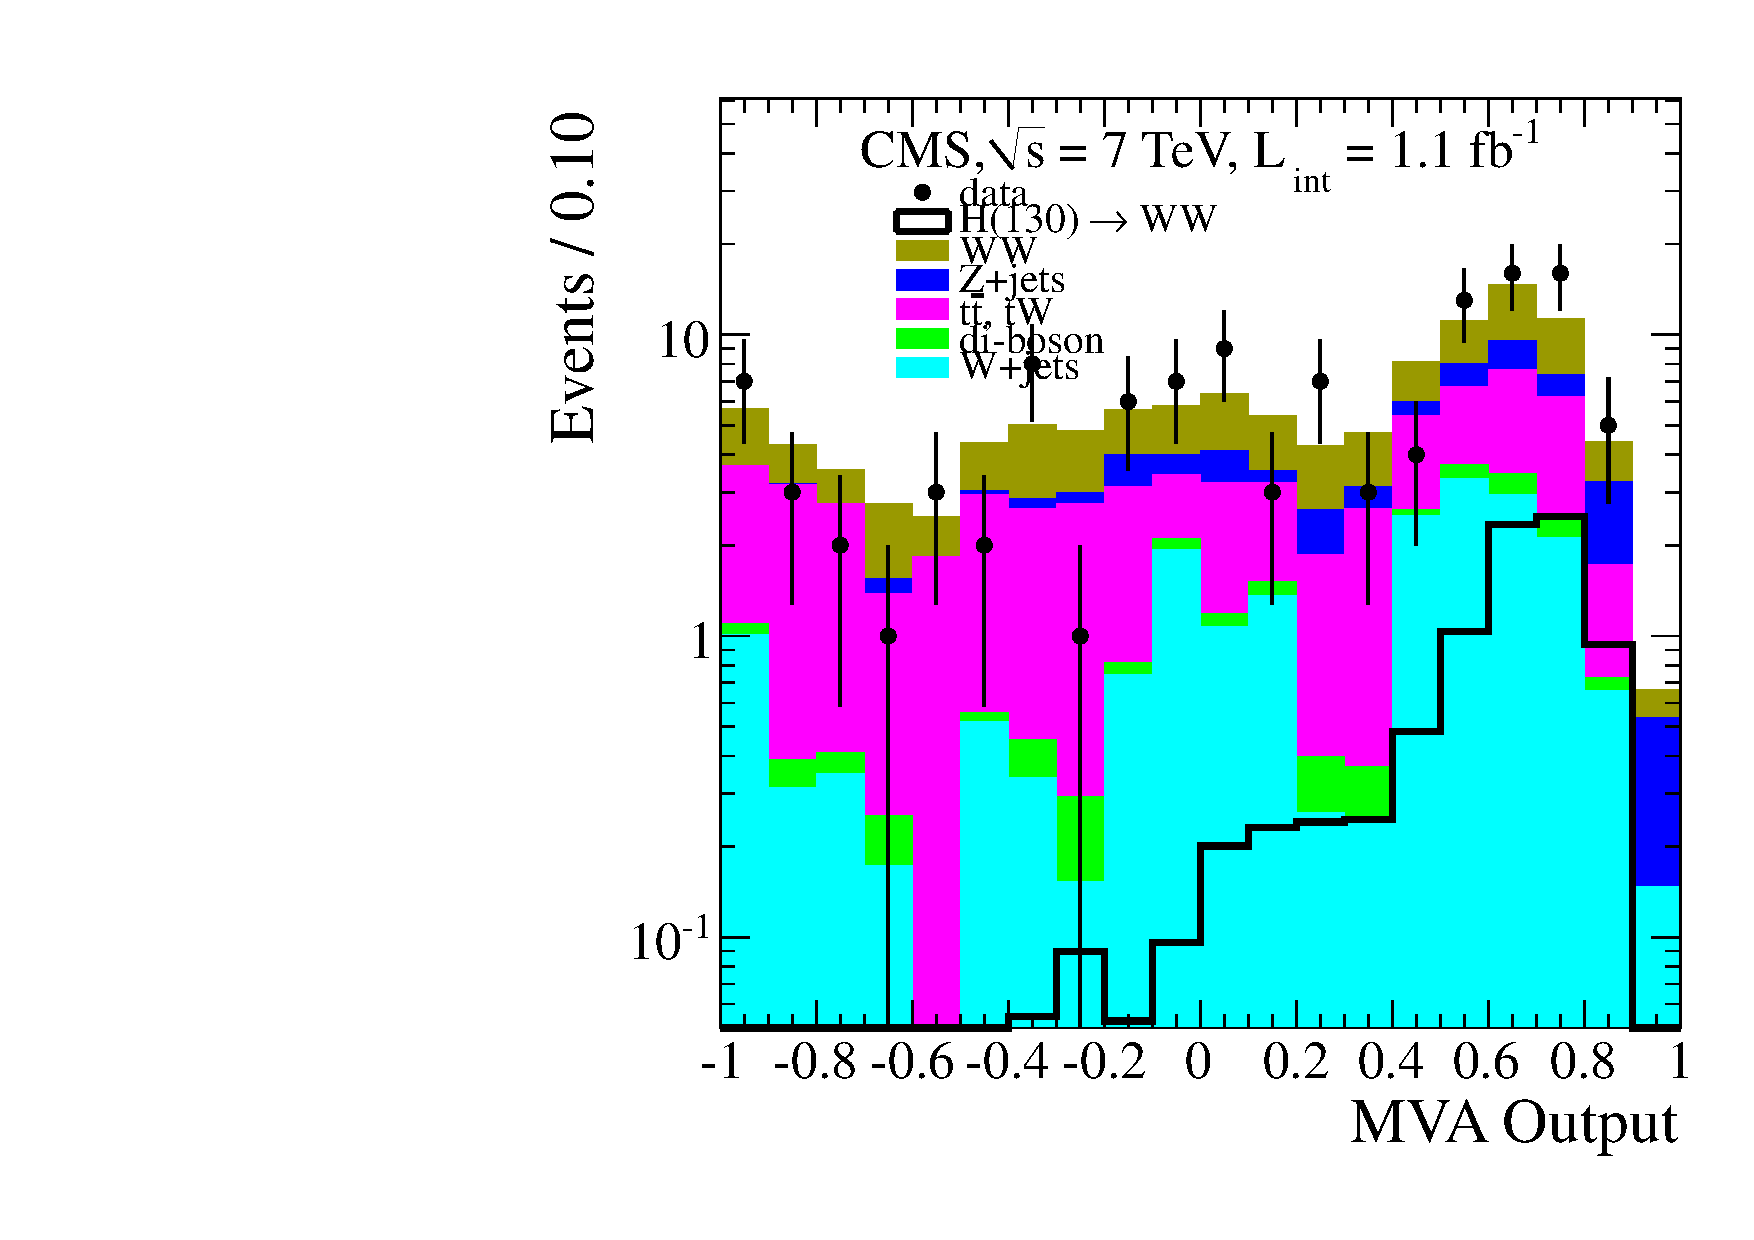
\includegraphics[width=0.49\textwidth,angle=0]{figures/histo_mva_130_1j_of.pdf}} 
       \caption{Classifier outputs for Higgs signal and background events 
for \mHi=130 $\GeVcc$ in the 0-jet bin same flavor final state (a), 1-jet bin same flavor final state (b), 
 0-jet bin opposite flavor final state (c), and 1-jet bin opposite flavor final state (d), after the $\WW$ selection. The number 
of events is different on each mass point due to the specific $\mll$ requirement.}
   \label{fig:histo_mva_130}
\end{center}
\end{figure}

\begin{figure}[!ht]
\begin{center}
   \subfigure[]{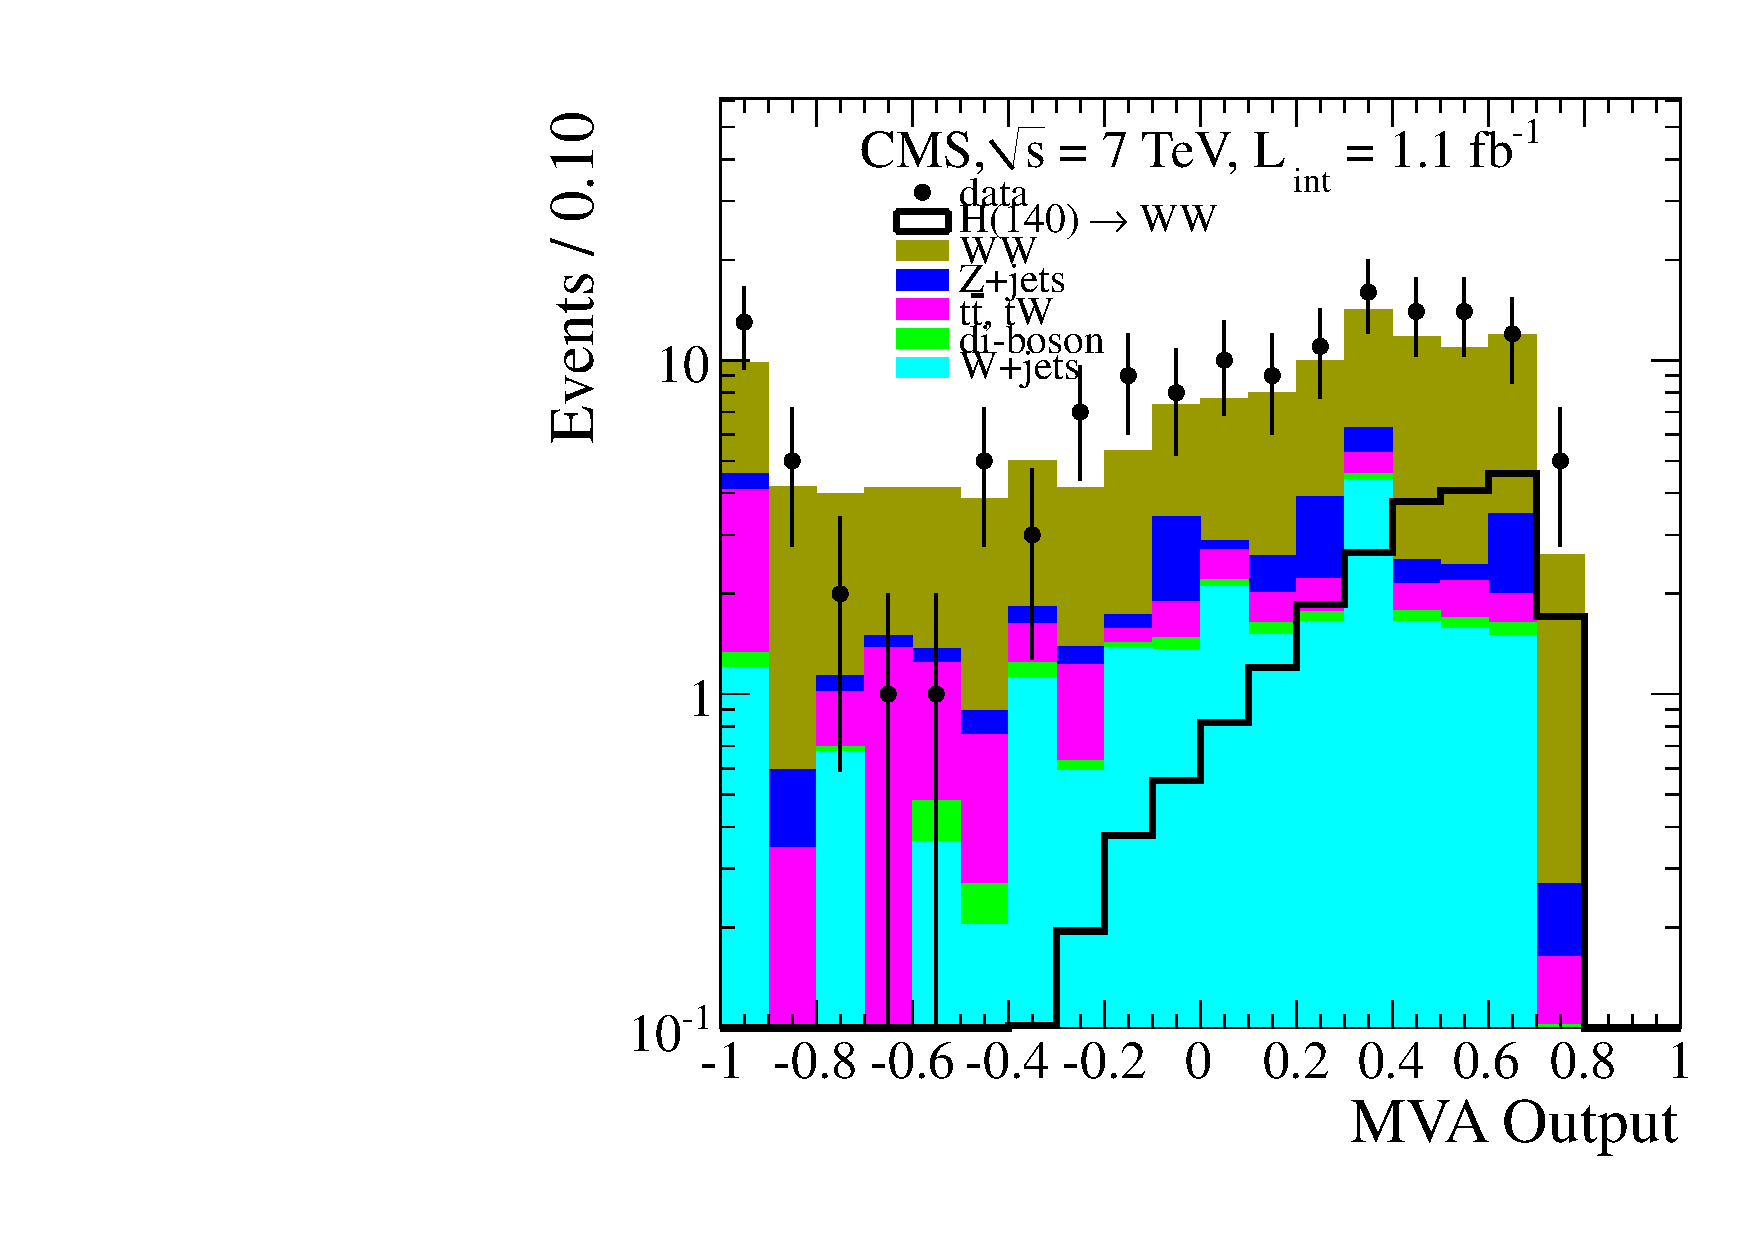
\includegraphics[width=0.49\textwidth,angle=0]{figures/histo_mva_140_0j_sf.pdf}} 
   \subfigure[]{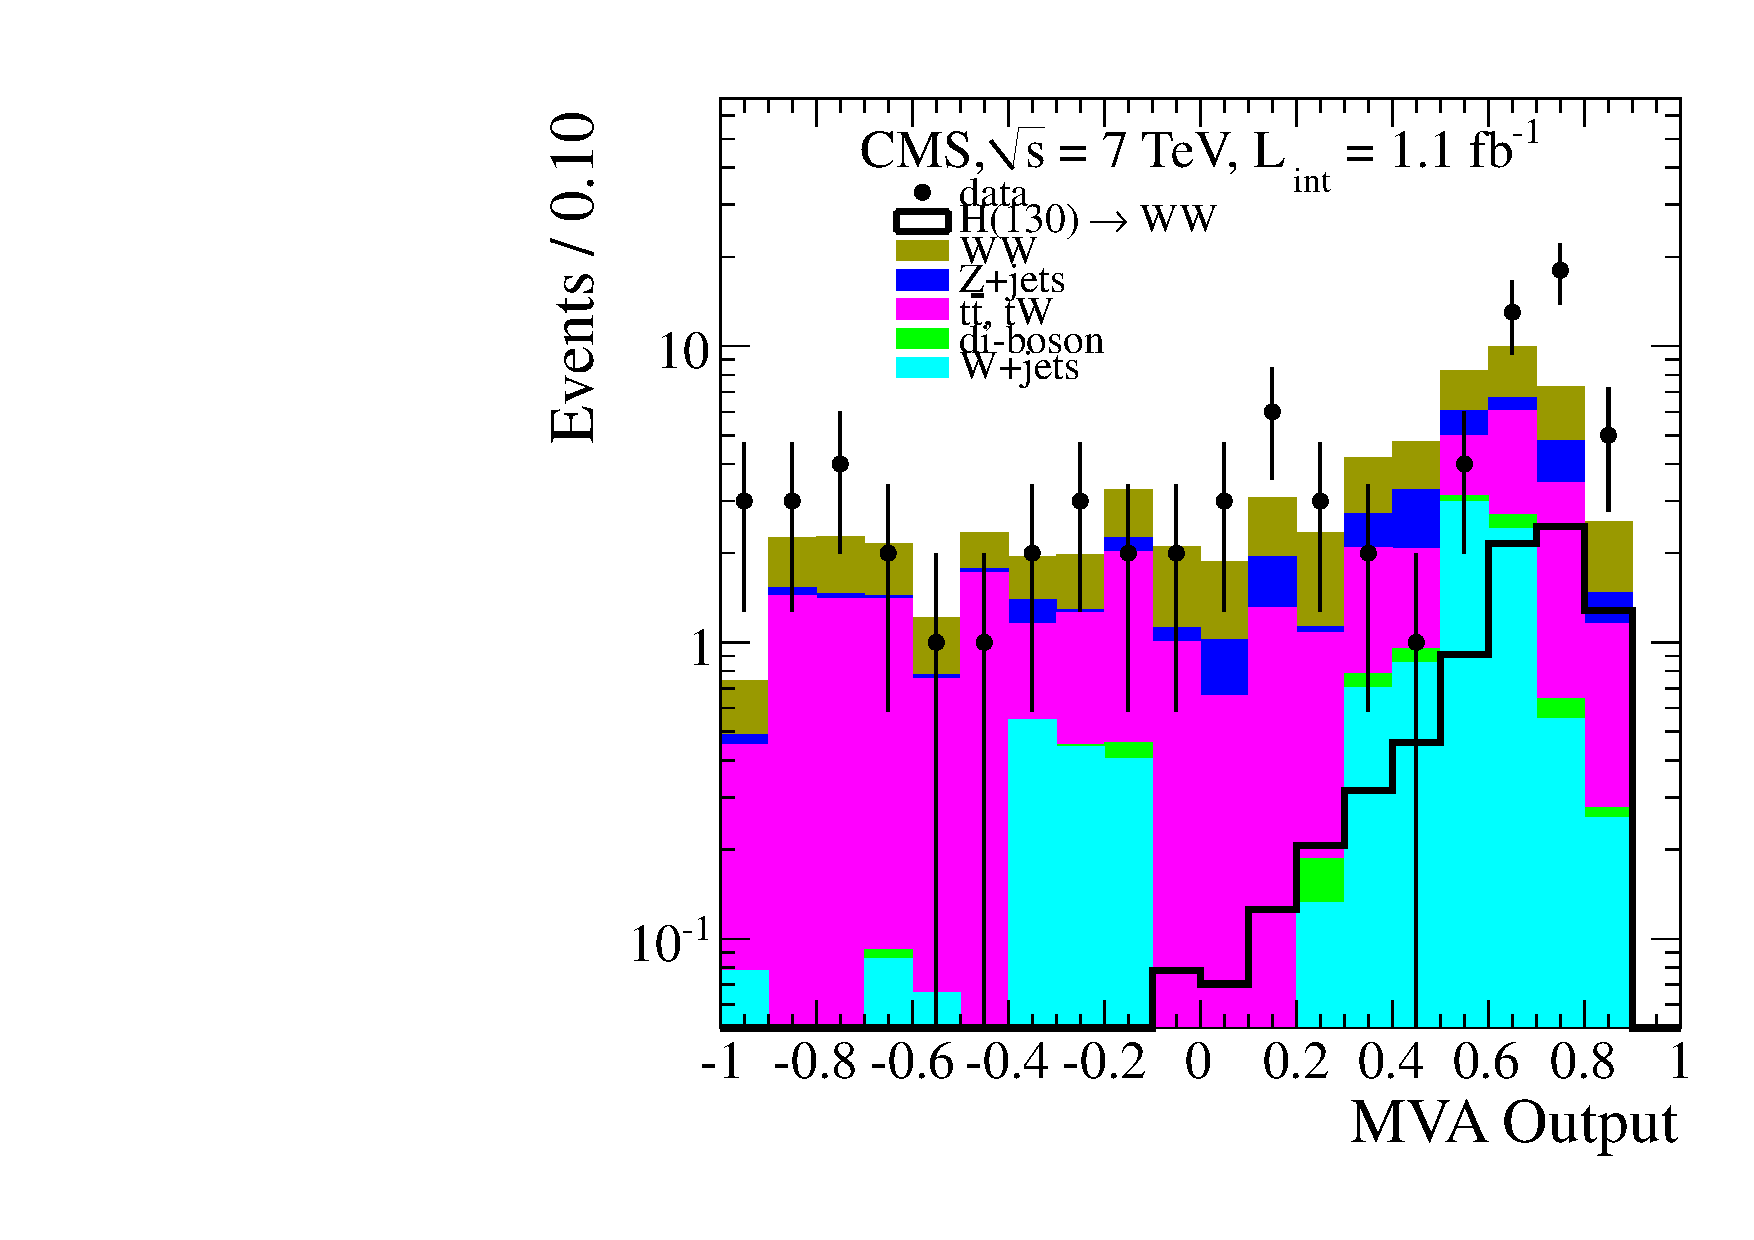
\includegraphics[width=0.49\textwidth,angle=0]{figures/histo_mva_140_1j_sf.pdf}} \\
   \subfigure[]{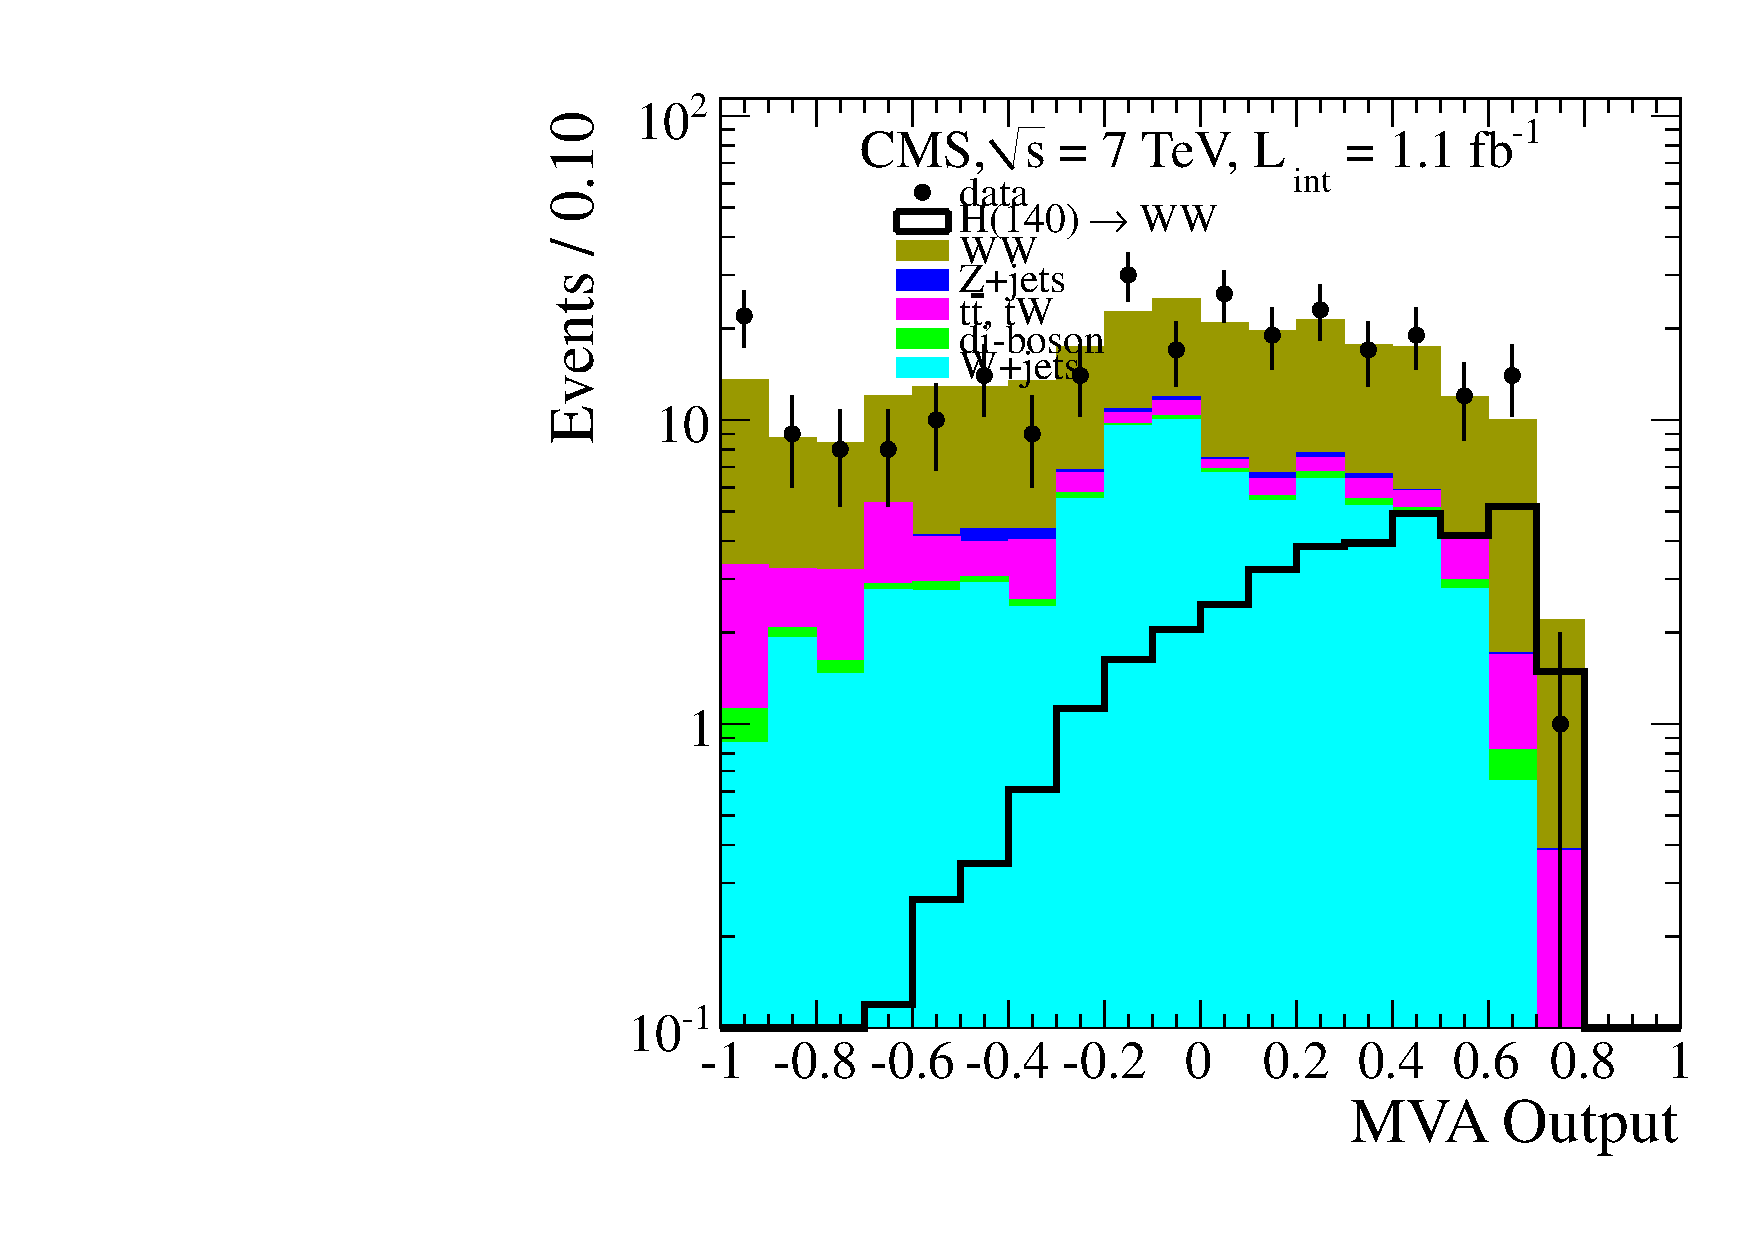
\includegraphics[width=0.49\textwidth,angle=0]{figures/histo_mva_140_0j_of.pdf}} 
   \subfigure[]{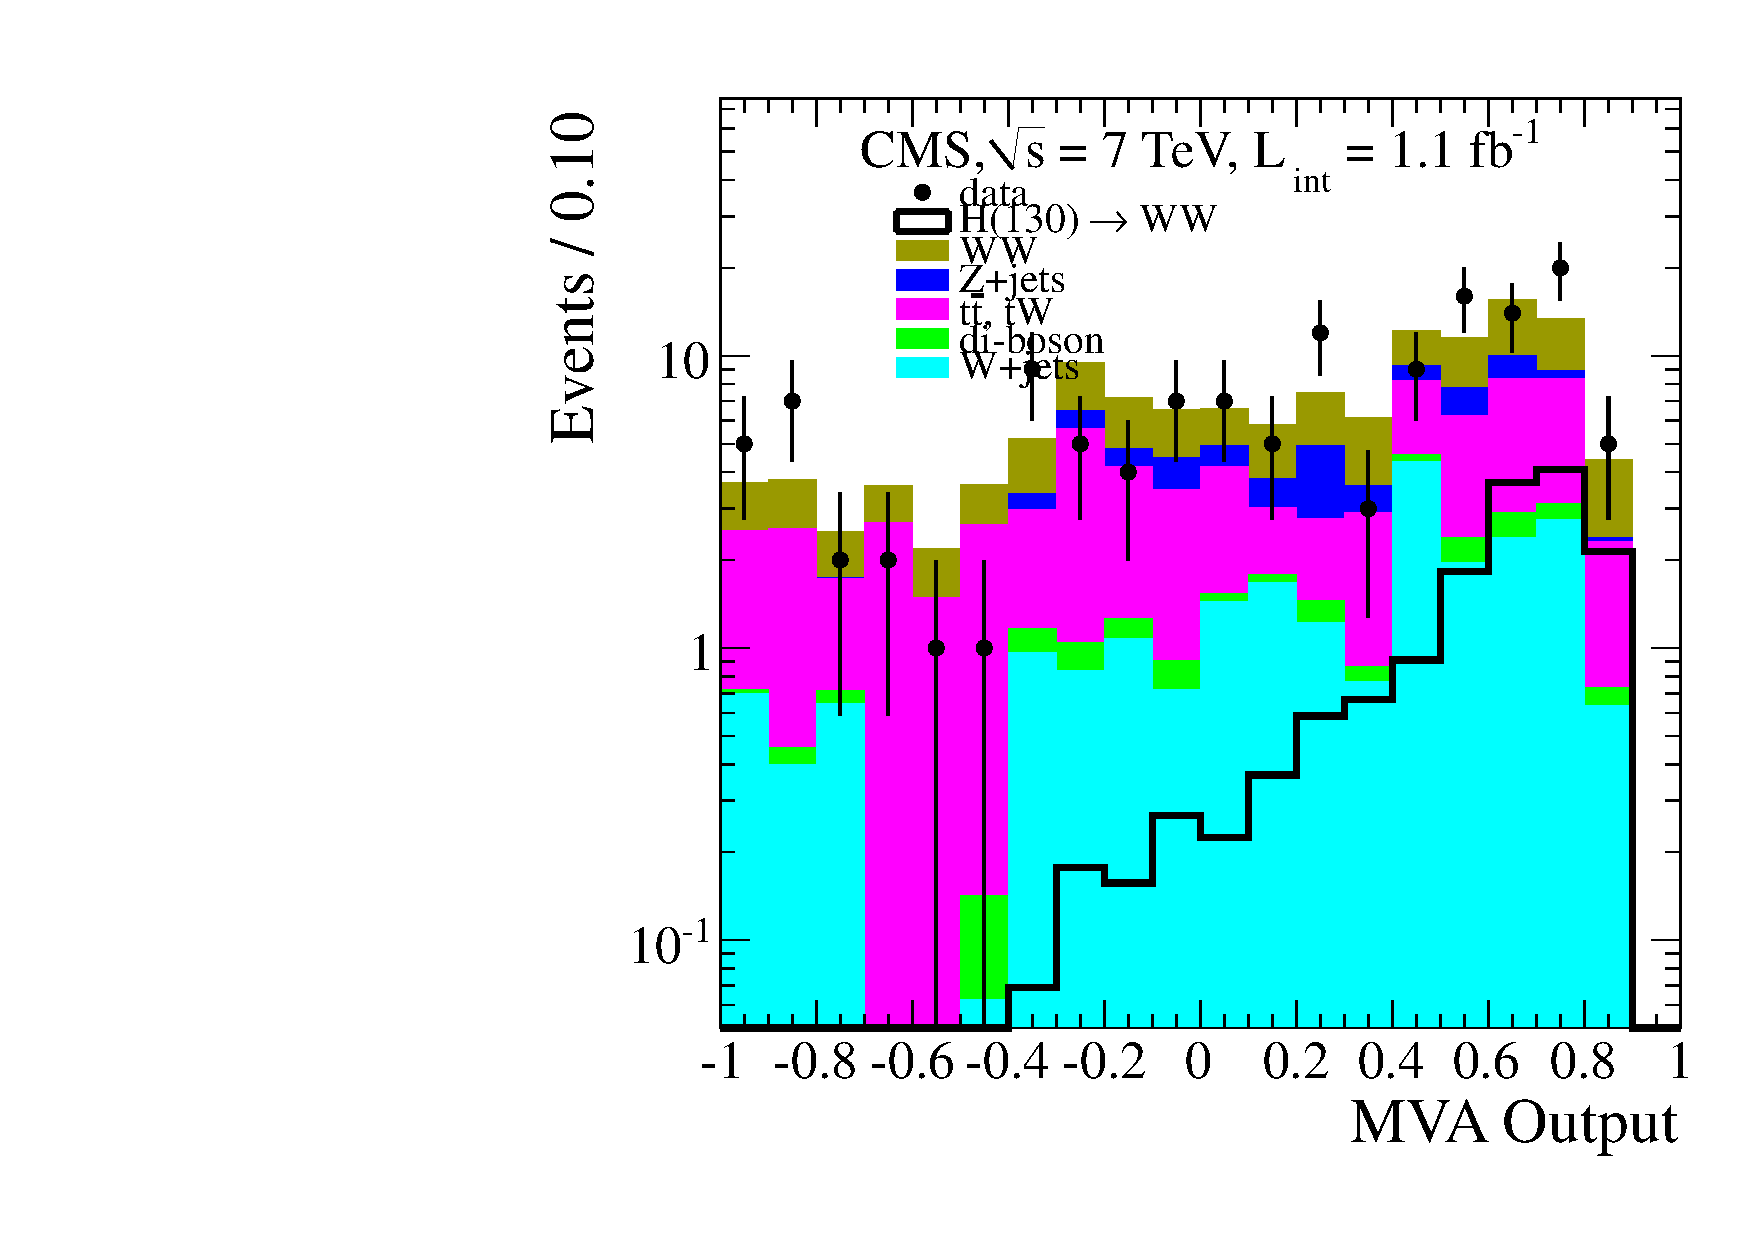
\includegraphics[width=0.49\textwidth,angle=0]{figures/histo_mva_140_1j_of.pdf}} 
       \caption{Classifier outputs for Higgs signal and background events 
for \mHi=140 $\GeVcc$ in the 0-jet bin same flavor final state (a), 1-jet bin same flavor final state (b), 
 0-jet bin opposite flavor final state (c), and 1-jet bin opposite flavor final state (d), after the $\WW$ selection. The number 
of events is different on each mass point due to the specific $\mll$ requirement.}
   \label{fig:histo_mva_140}
\end{center}
\end{figure}

\begin{figure}[!ht]
\begin{center}
   \subfigure[]{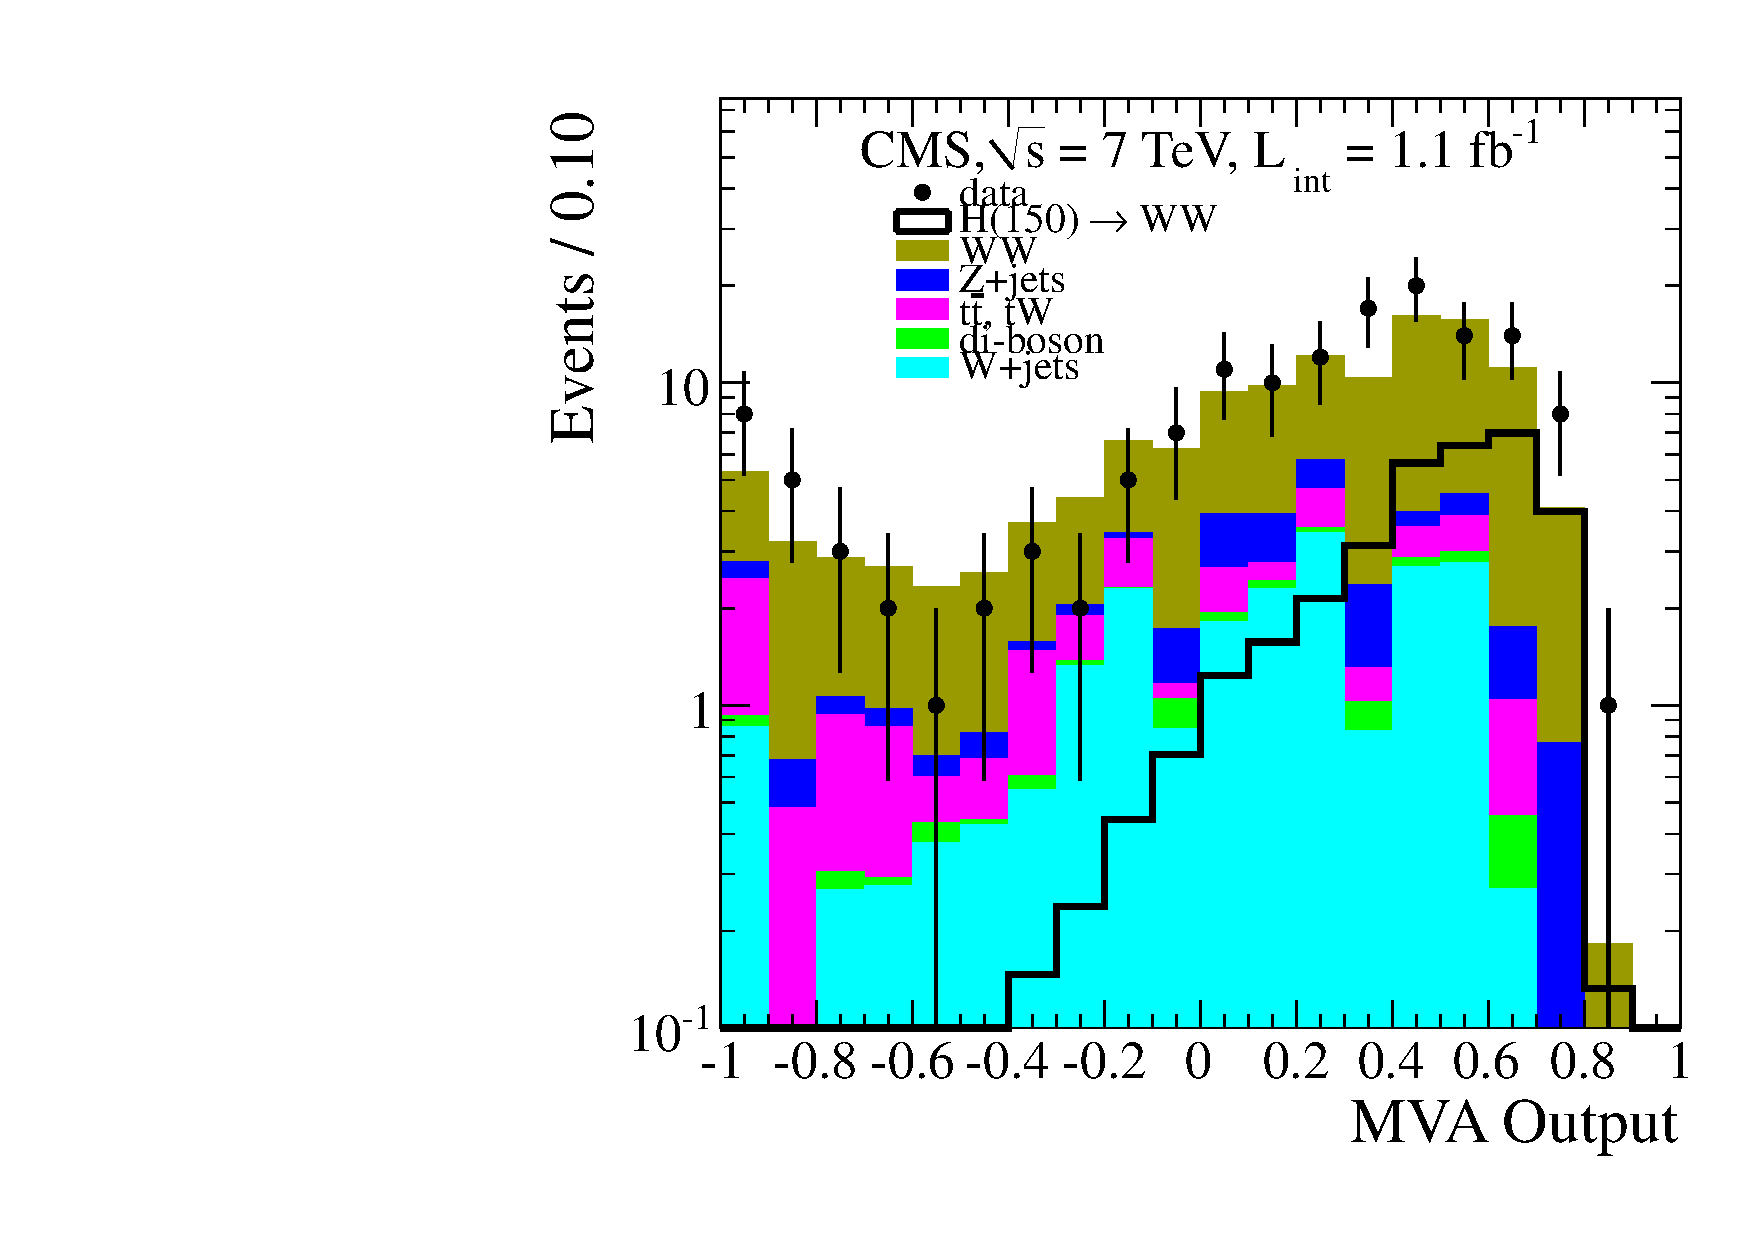
\includegraphics[width=0.49\textwidth,angle=0]{figures/histo_mva_150_0j_sf.pdf}} 
   \subfigure[]{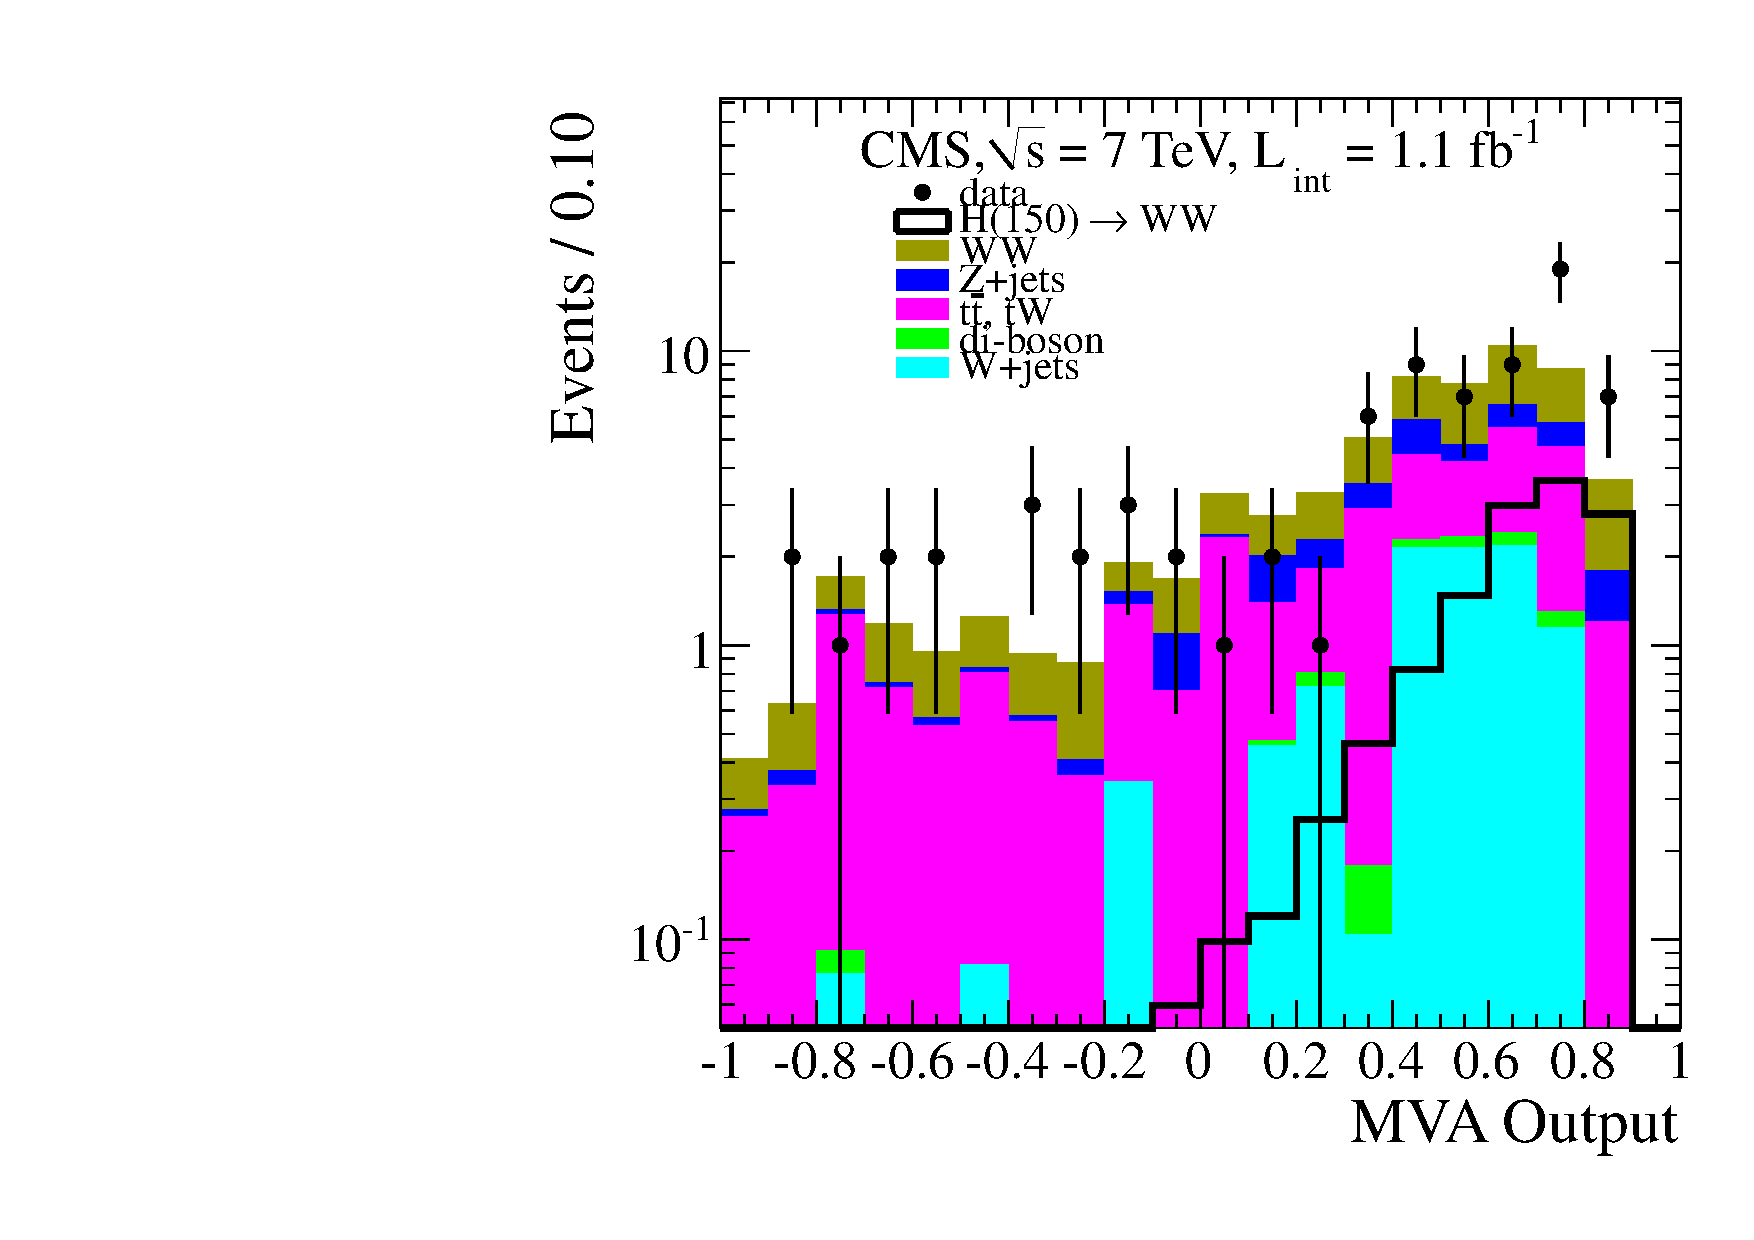
\includegraphics[width=0.49\textwidth,angle=0]{figures/histo_mva_150_1j_sf.pdf}}  \\
   \subfigure[]{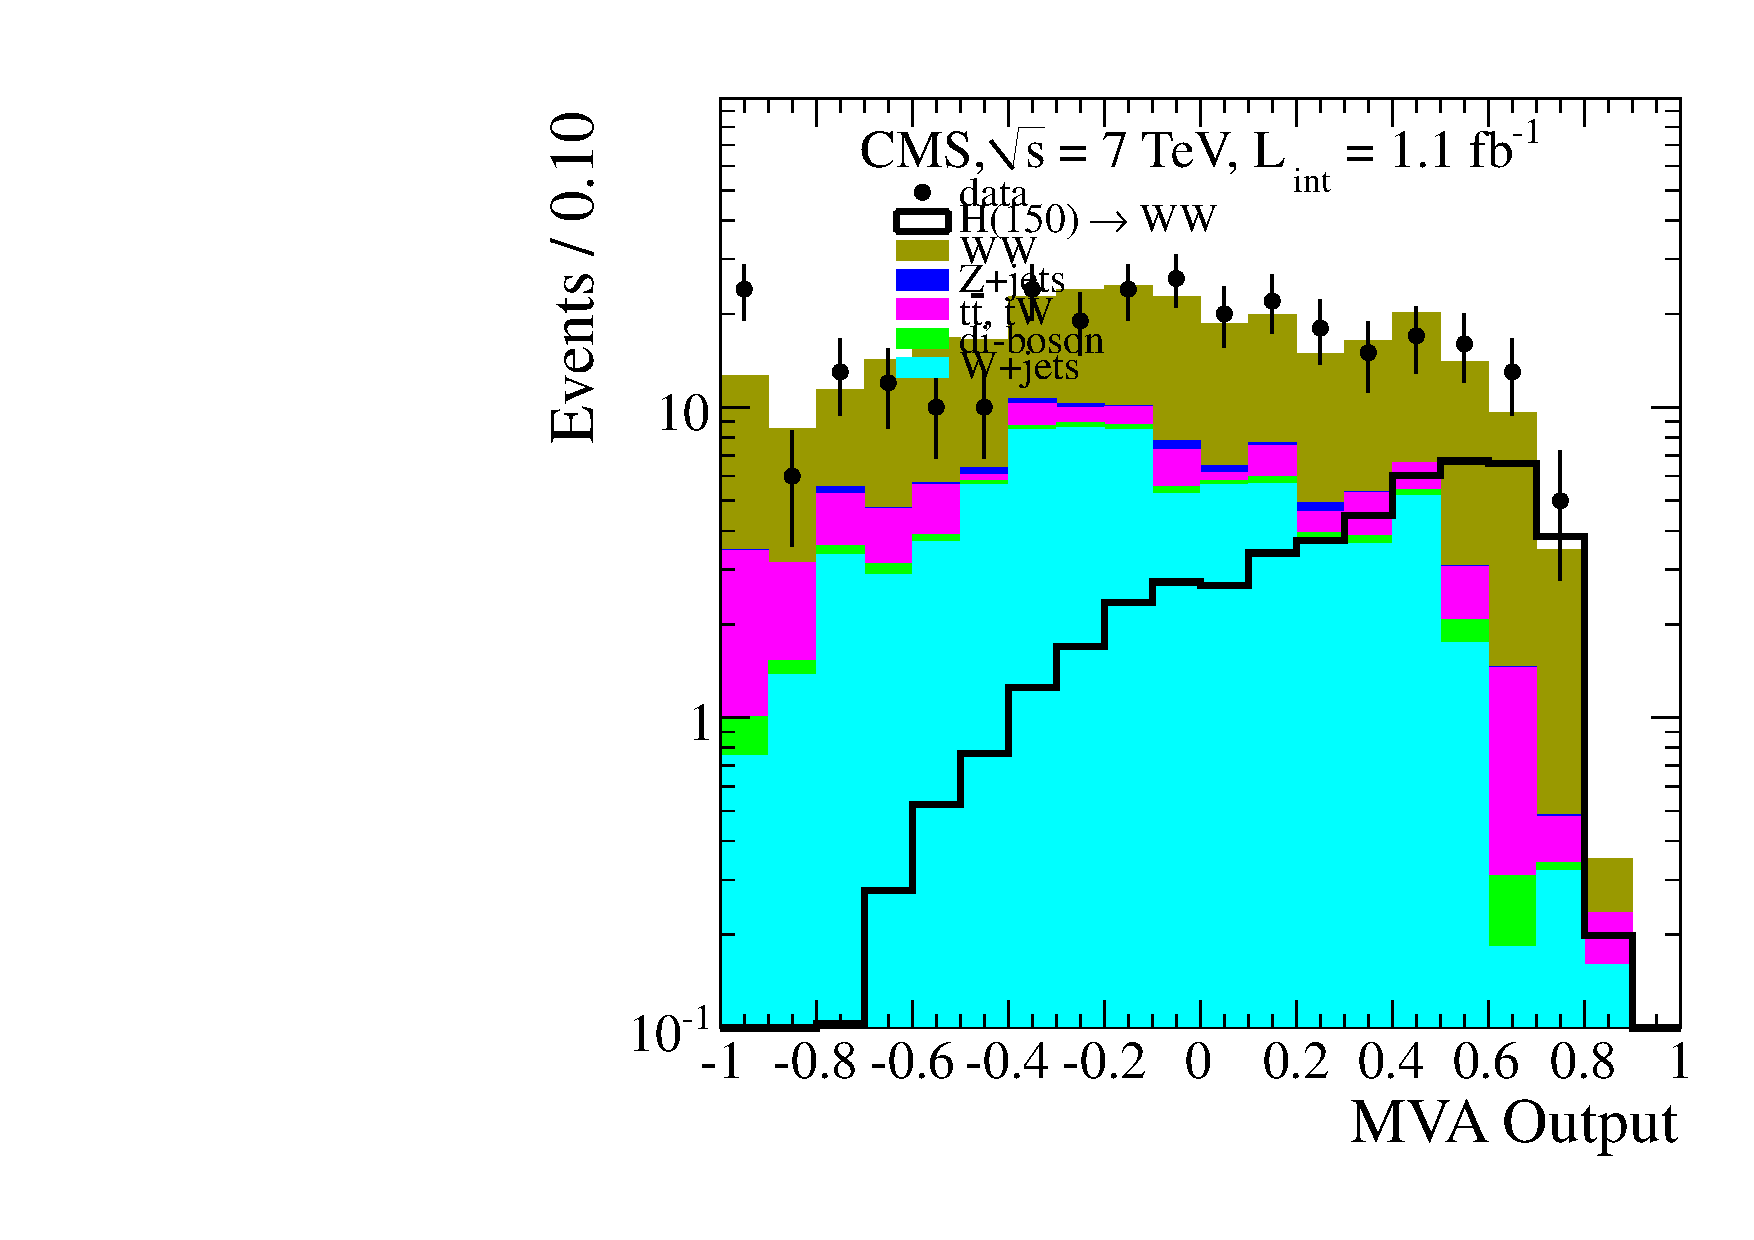
\includegraphics[width=0.49\textwidth,angle=0]{figures/histo_mva_150_0j_of.pdf}} 
   \subfigure[]{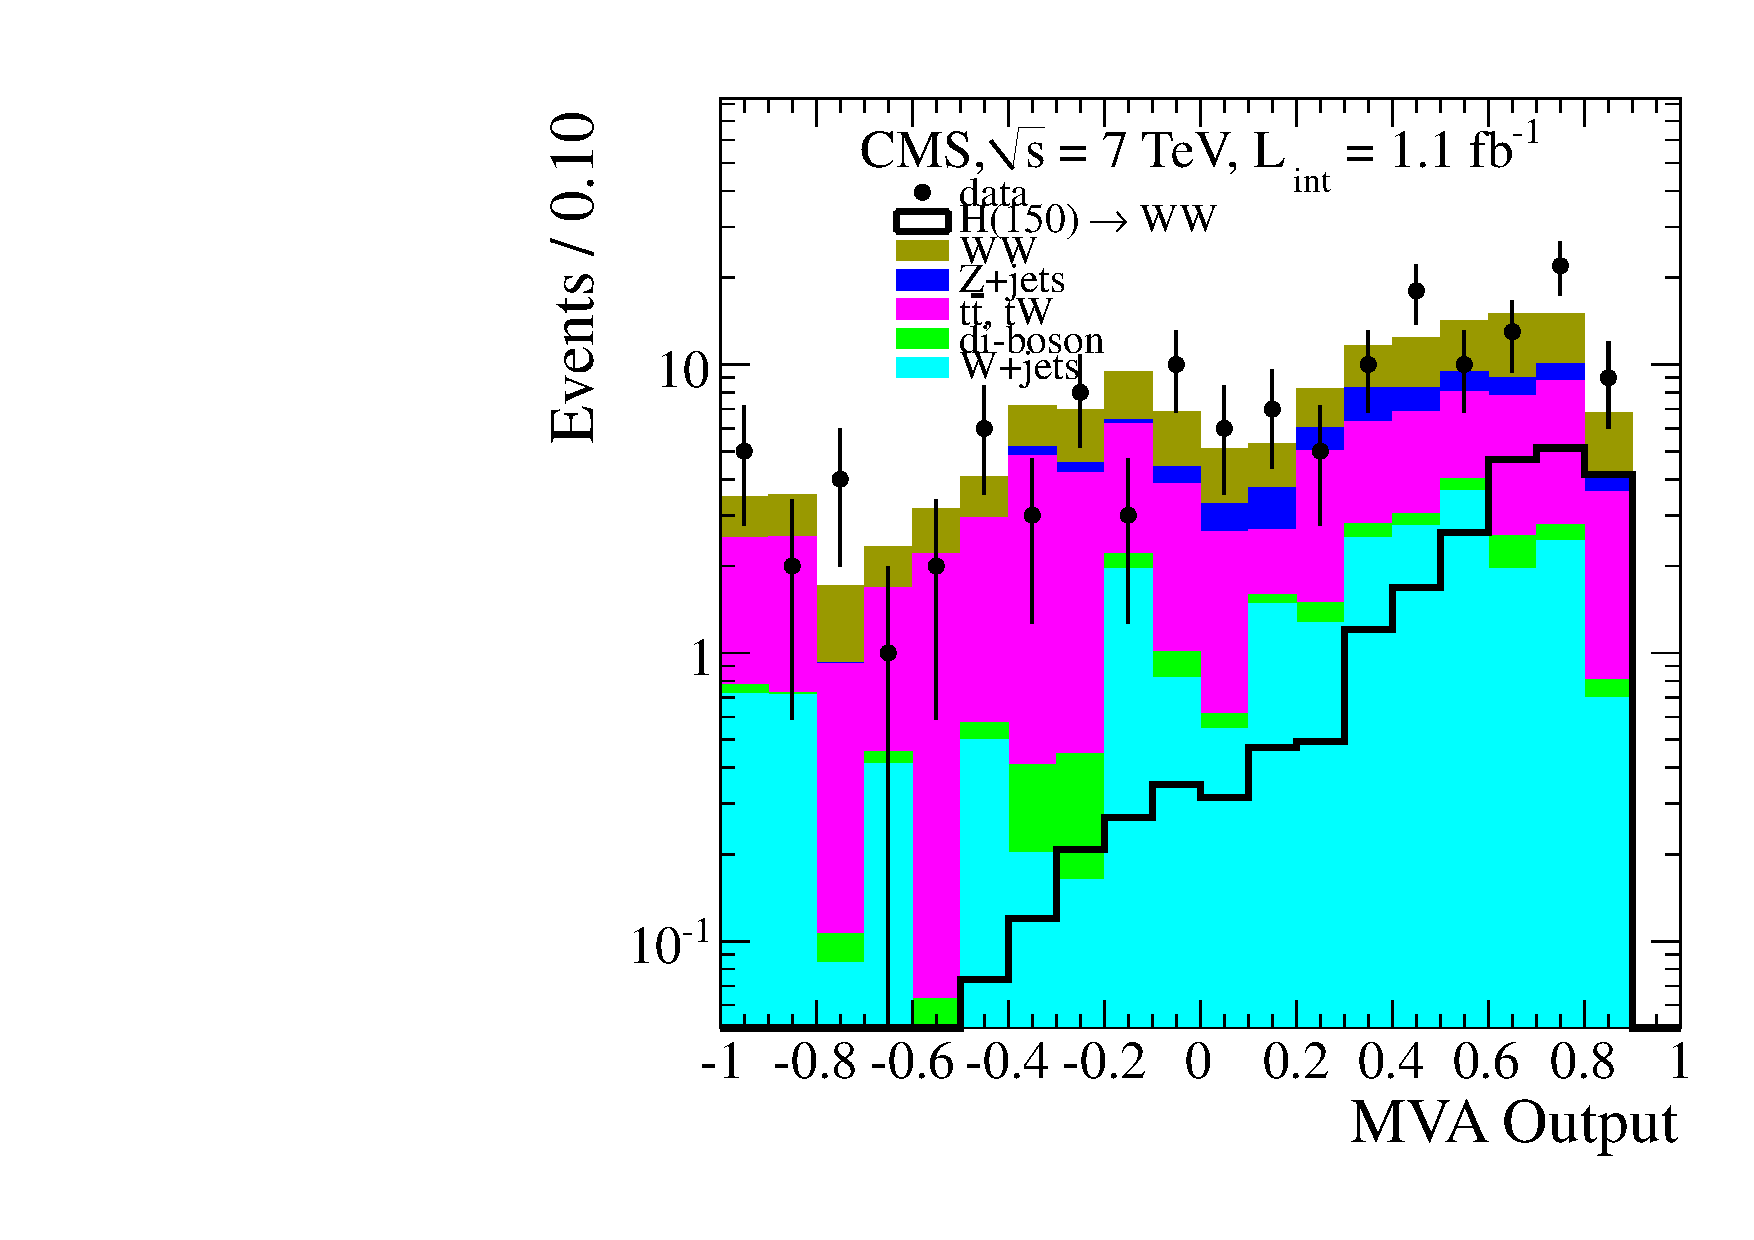
\includegraphics[width=0.49\textwidth,angle=0]{figures/histo_mva_150_1j_of.pdf}} 
       \caption{Classifier outputs for Higgs signal and background events 
for \mHi=150 $\GeVcc$ in the 0-jet bin same flavor final state (a), 1-jet bin same flavor final state (b), 
 0-jet bin opposite flavor final state (c), and 1-jet bin opposite flavor final state (d), after the $\WW$ selection. The number 
of events is different on each mass point due to the specific $\mll$ requirement.}
   \label{fig:histo_mva_150}
\end{center}
\end{figure}

\begin{figure}[!ht]
\begin{center}
   \subfigure[]{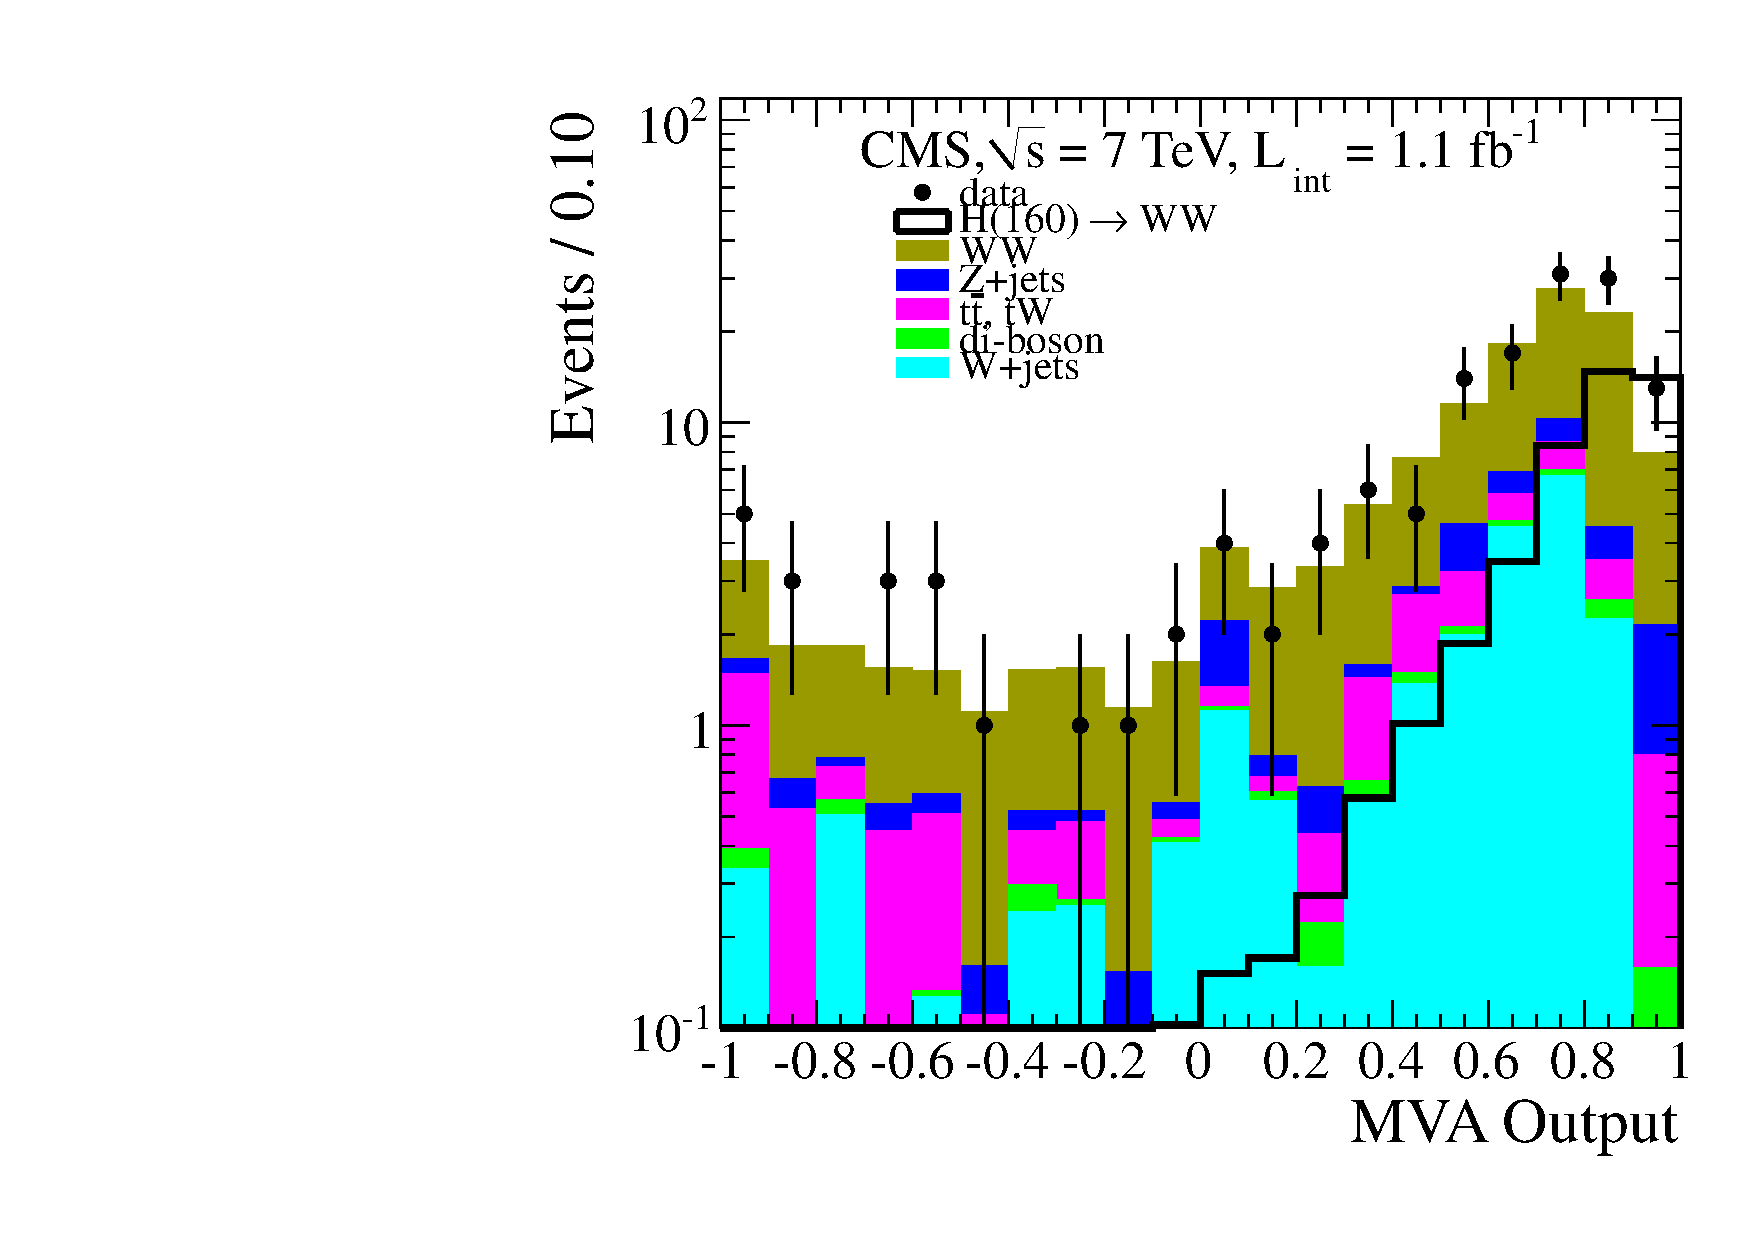
\includegraphics[width=0.49\textwidth,angle=0]{figures/histo_mva_160_0j_sf.pdf}} 
   \subfigure[]{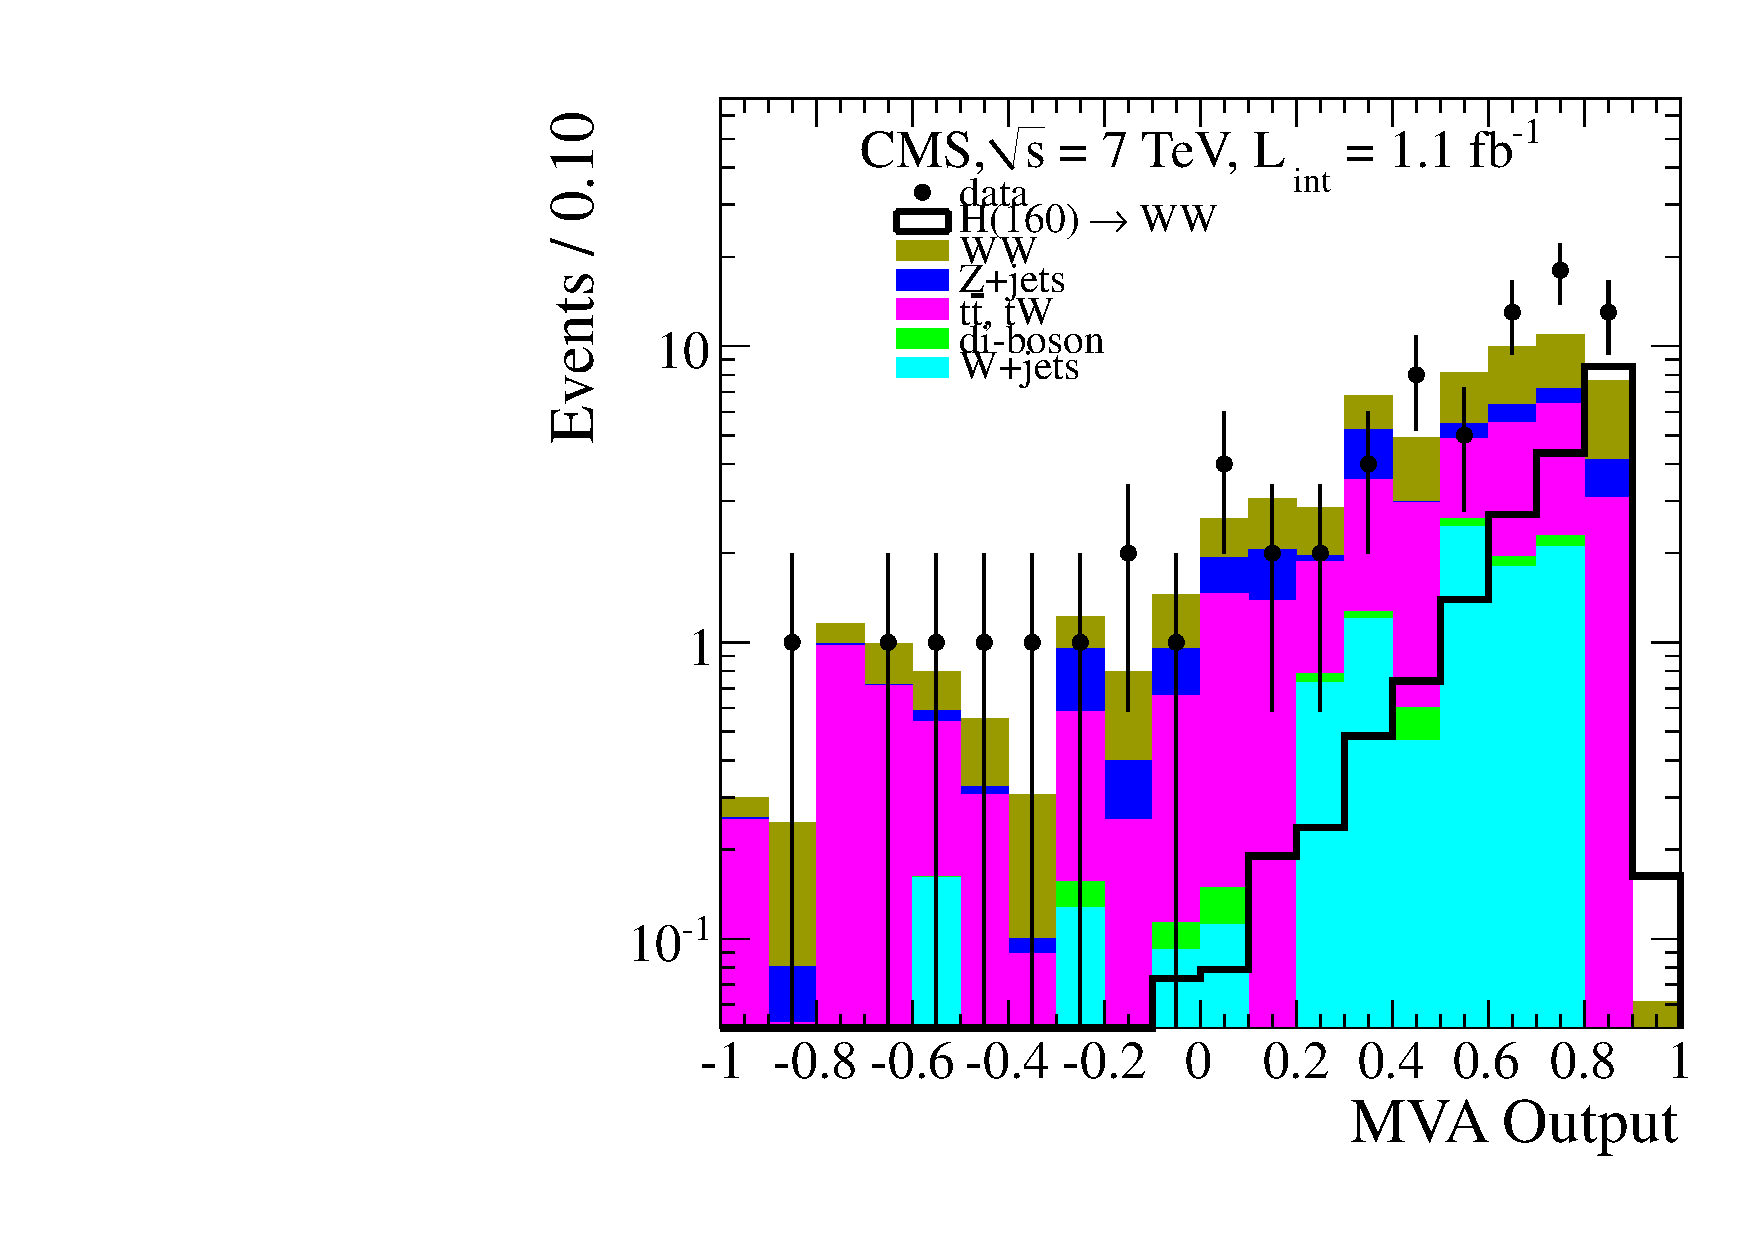
\includegraphics[width=0.49\textwidth,angle=0]{figures/histo_mva_160_1j_sf.pdf}}  \\
   \subfigure[]{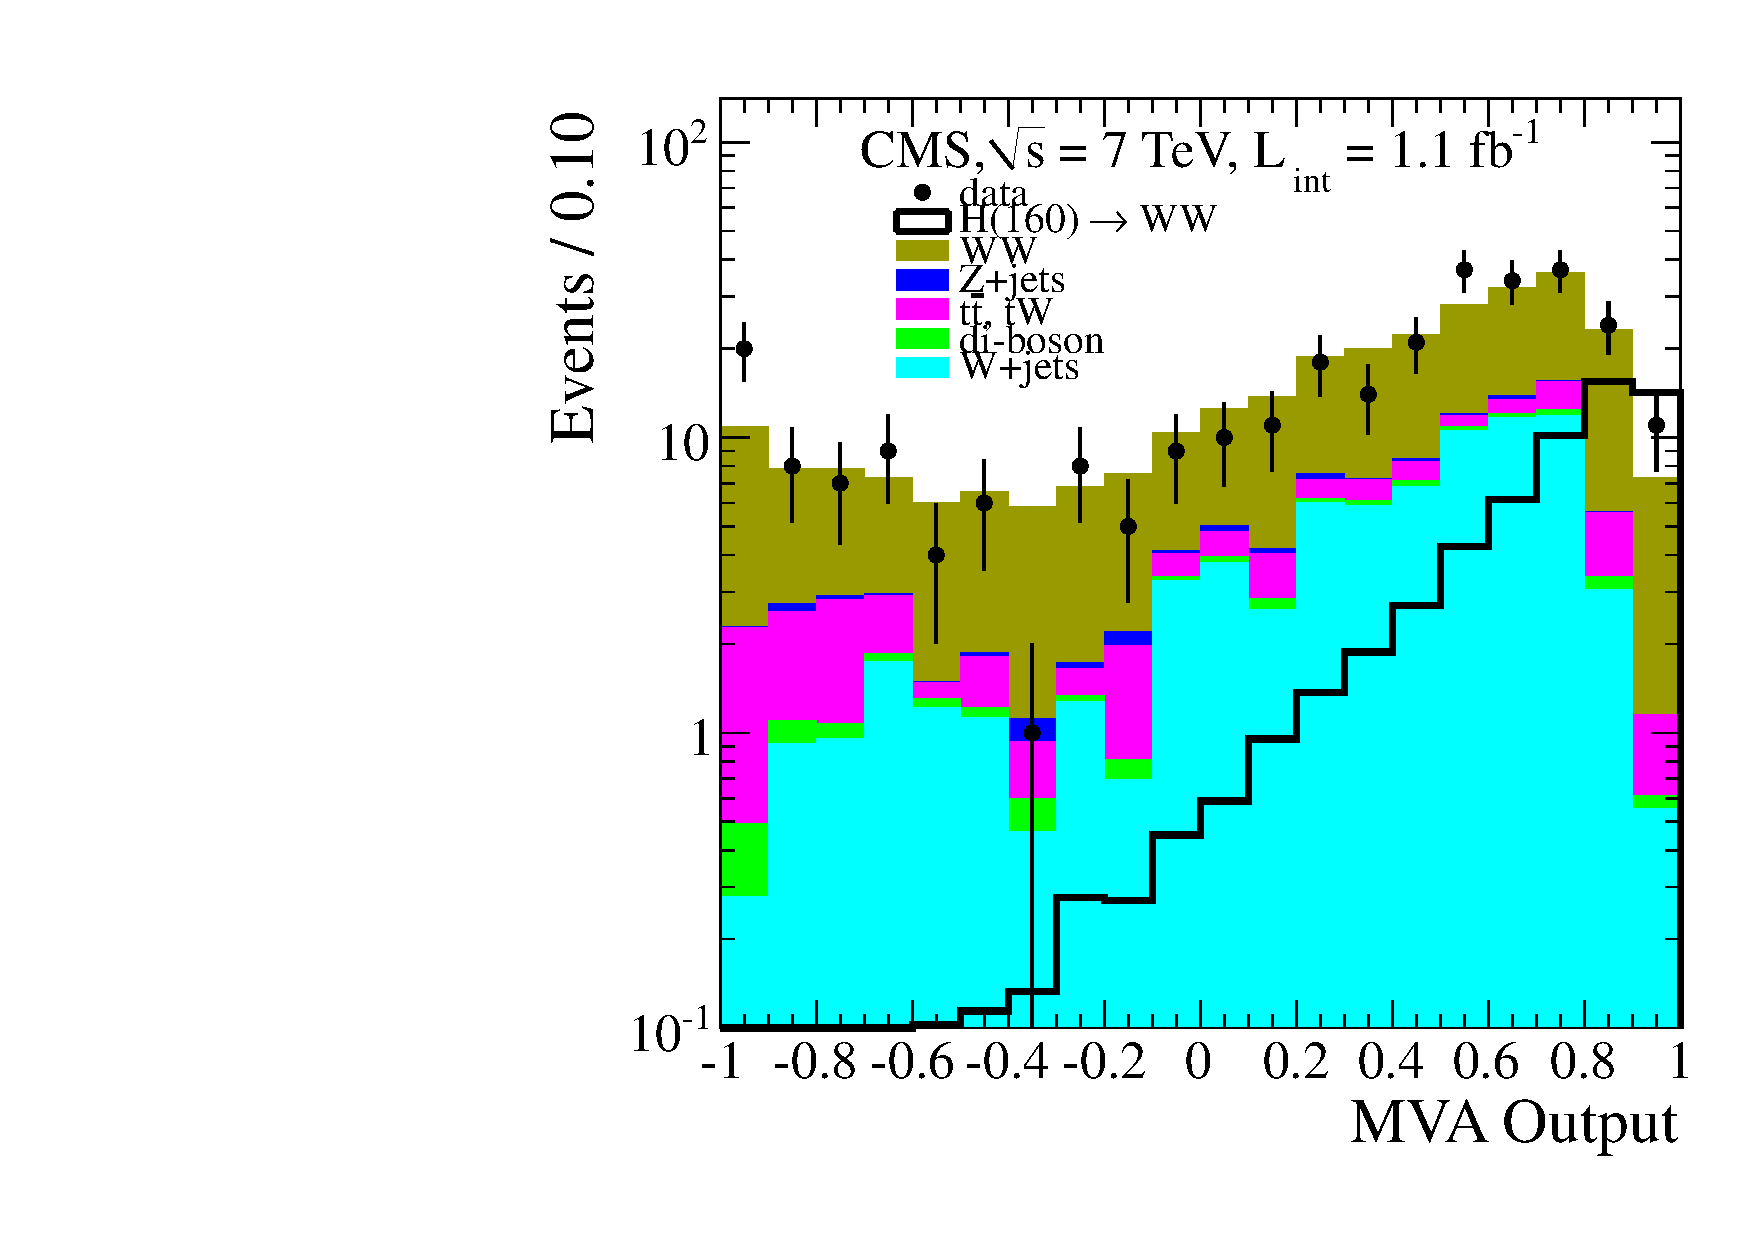
\includegraphics[width=0.49\textwidth,angle=0]{figures/histo_mva_160_0j_of.pdf}} 
   \subfigure[]{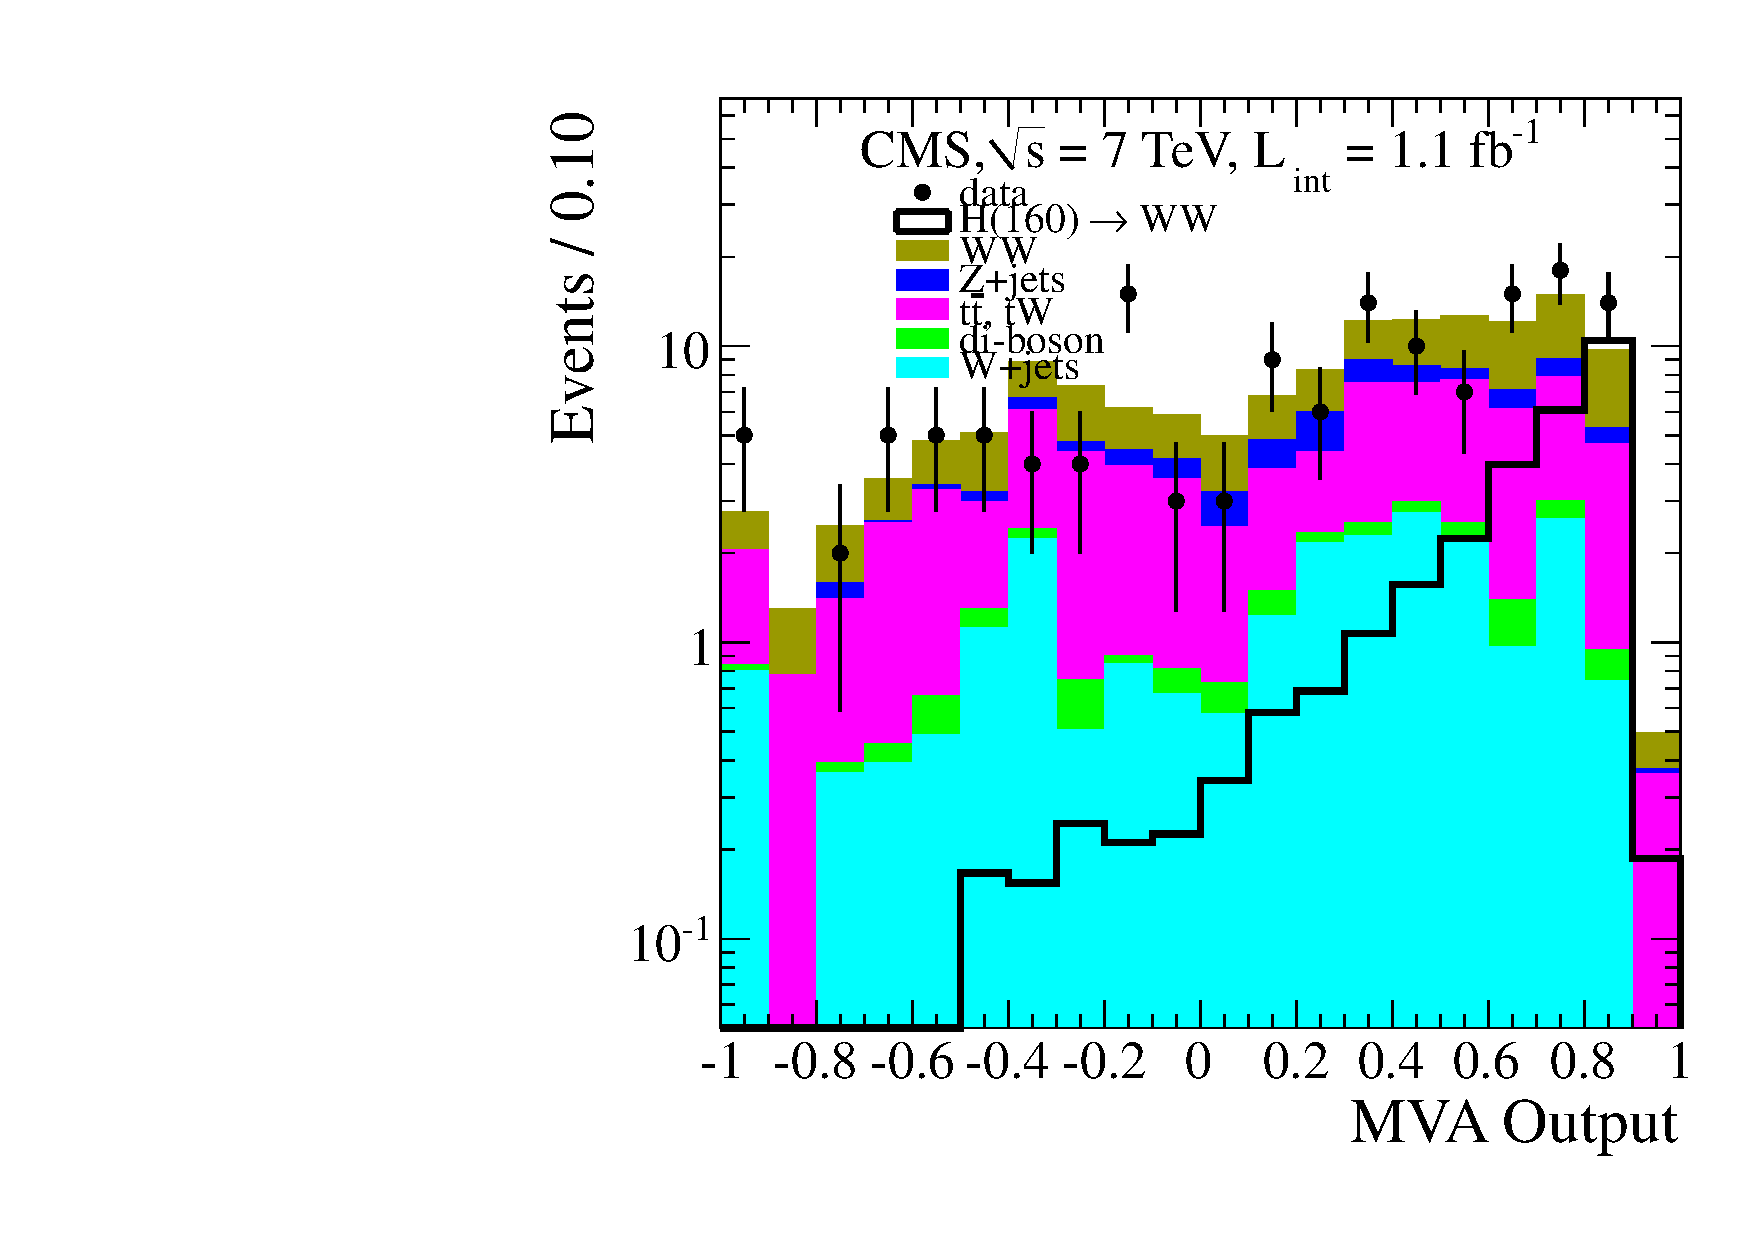
\includegraphics[width=0.49\textwidth,angle=0]{figures/histo_mva_160_1j_of.pdf}} 
       \caption{Classifier outputs for Higgs signal and background events 
for \mHi=160 $\GeVcc$ in the 0-jet bin same flavor final state (a), 1-jet bin same flavor final state (b), 
 0-jet bin opposite flavor final state (c), and 1-jet bin opposite flavor final state (d), after the $\WW$ selection. The number 
of events is different on each mass point due to the specific $\mll$ requirement.}
   \label{fig:histo_mva_160}
\end{center}
\end{figure}

\begin{figure}[!ht]
\begin{center}
   \subfigure[]{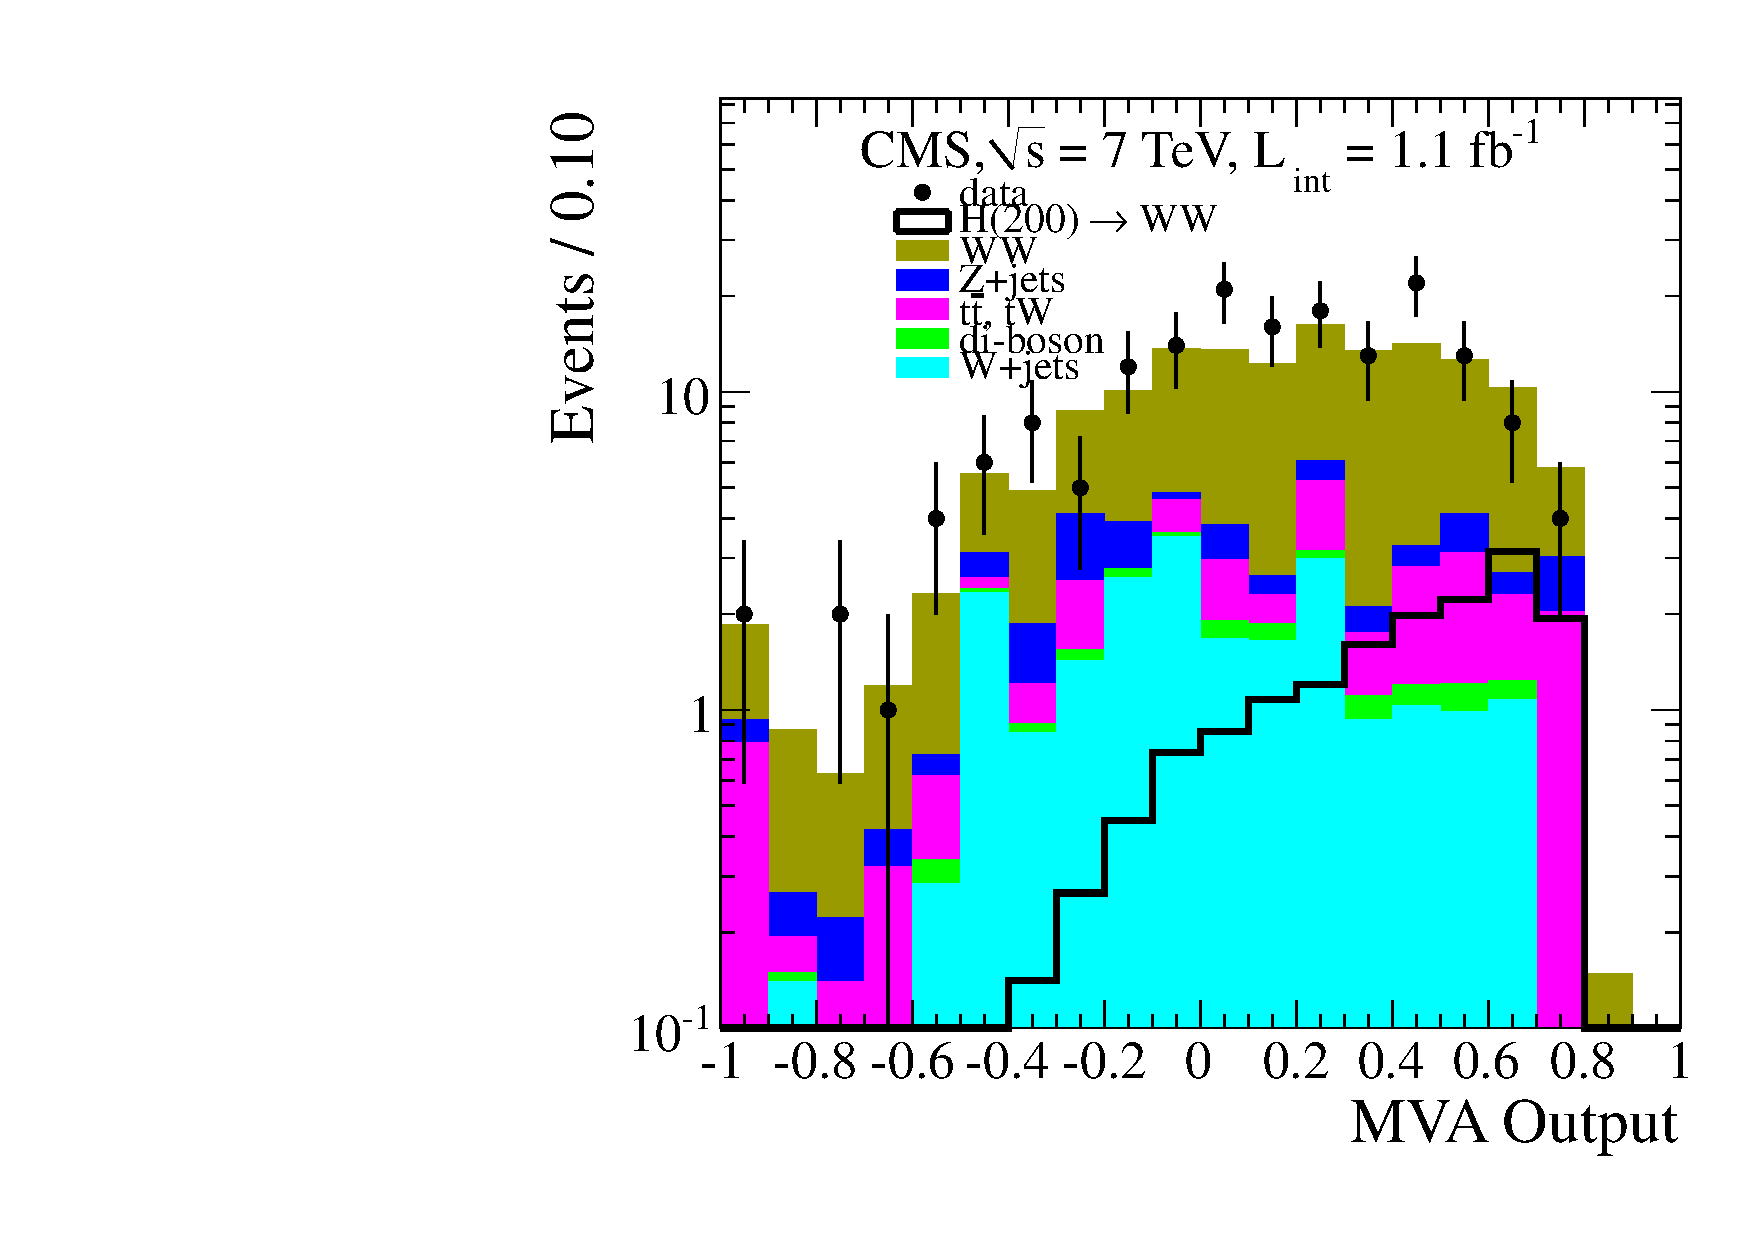
\includegraphics[width=0.49\textwidth,angle=0]{figures/histo_mva_200_0j_sf.pdf}} 
   \subfigure[]{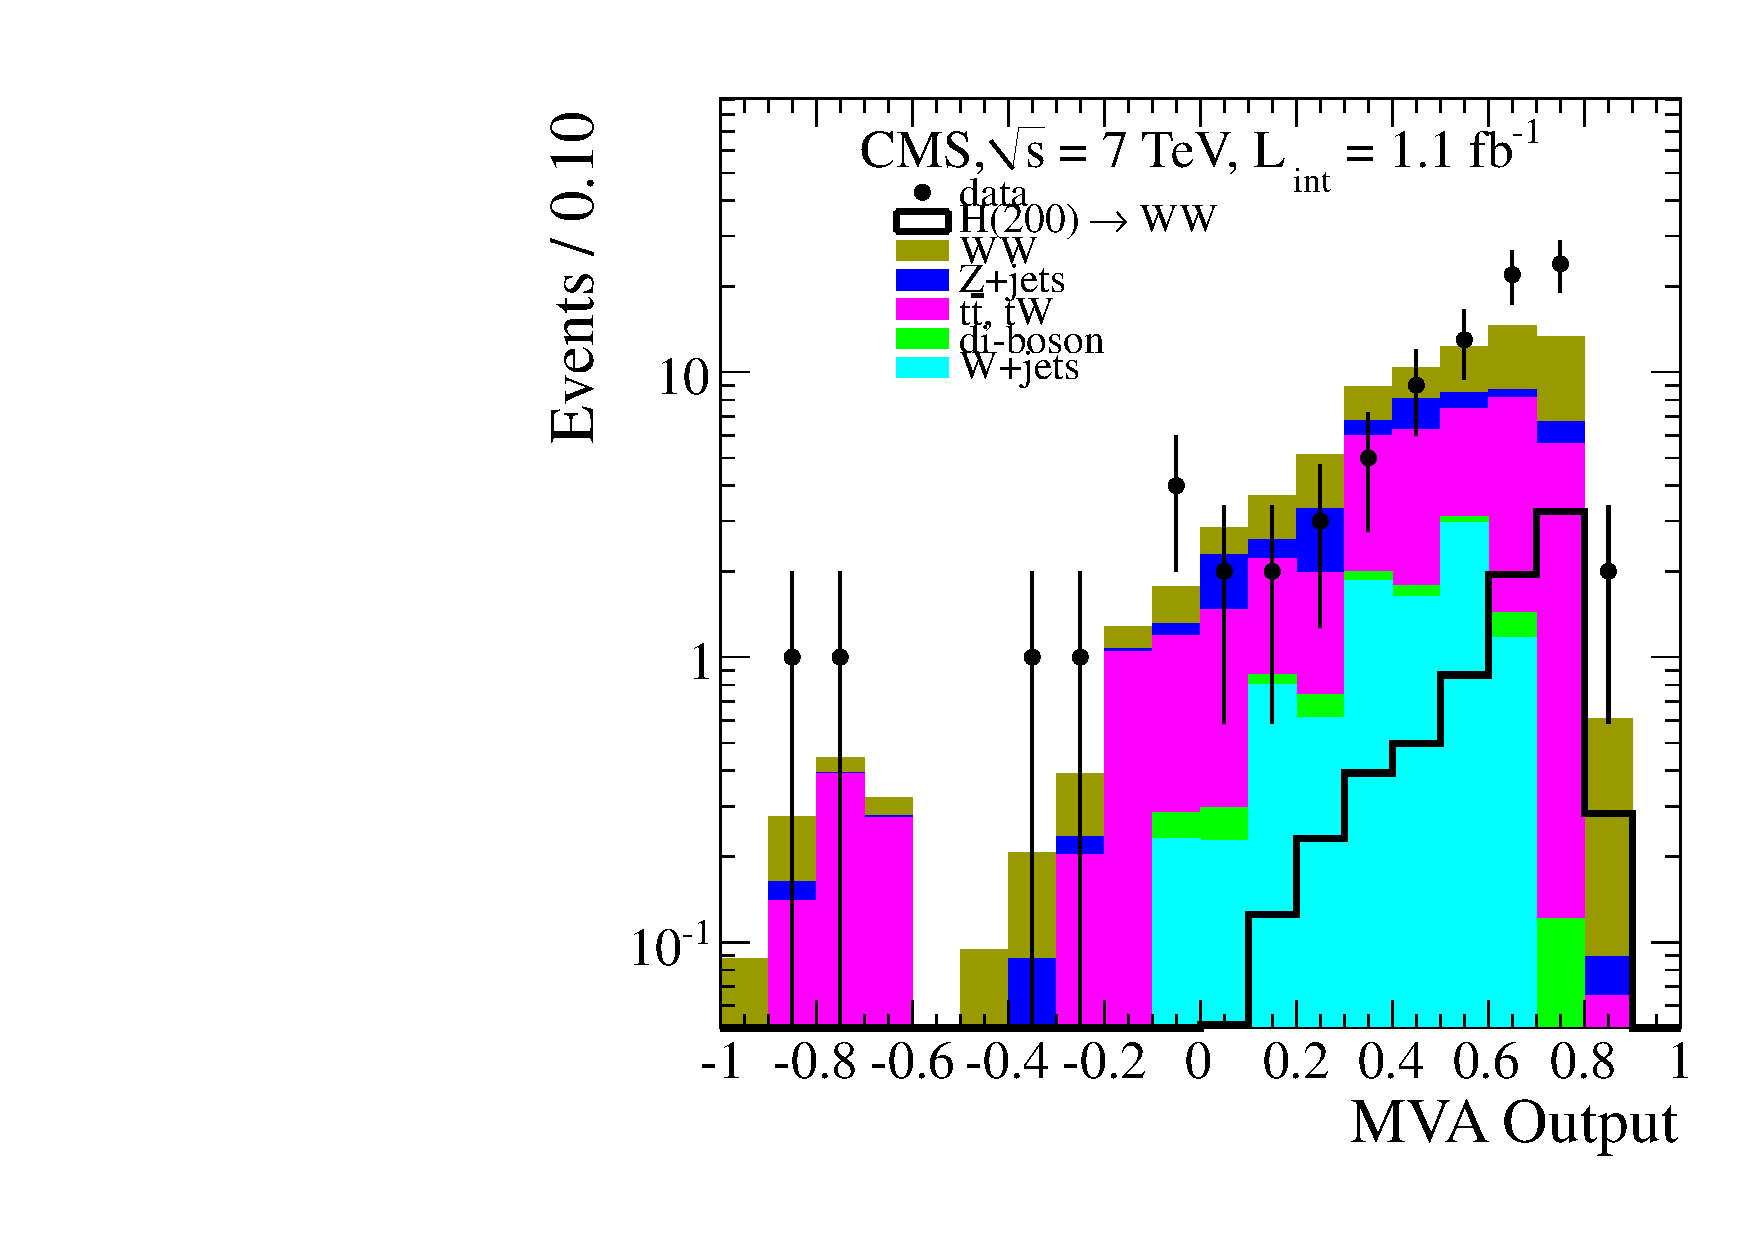
\includegraphics[width=0.49\textwidth,angle=0]{figures/histo_mva_200_1j_sf.pdf}}  \\
   \subfigure[]{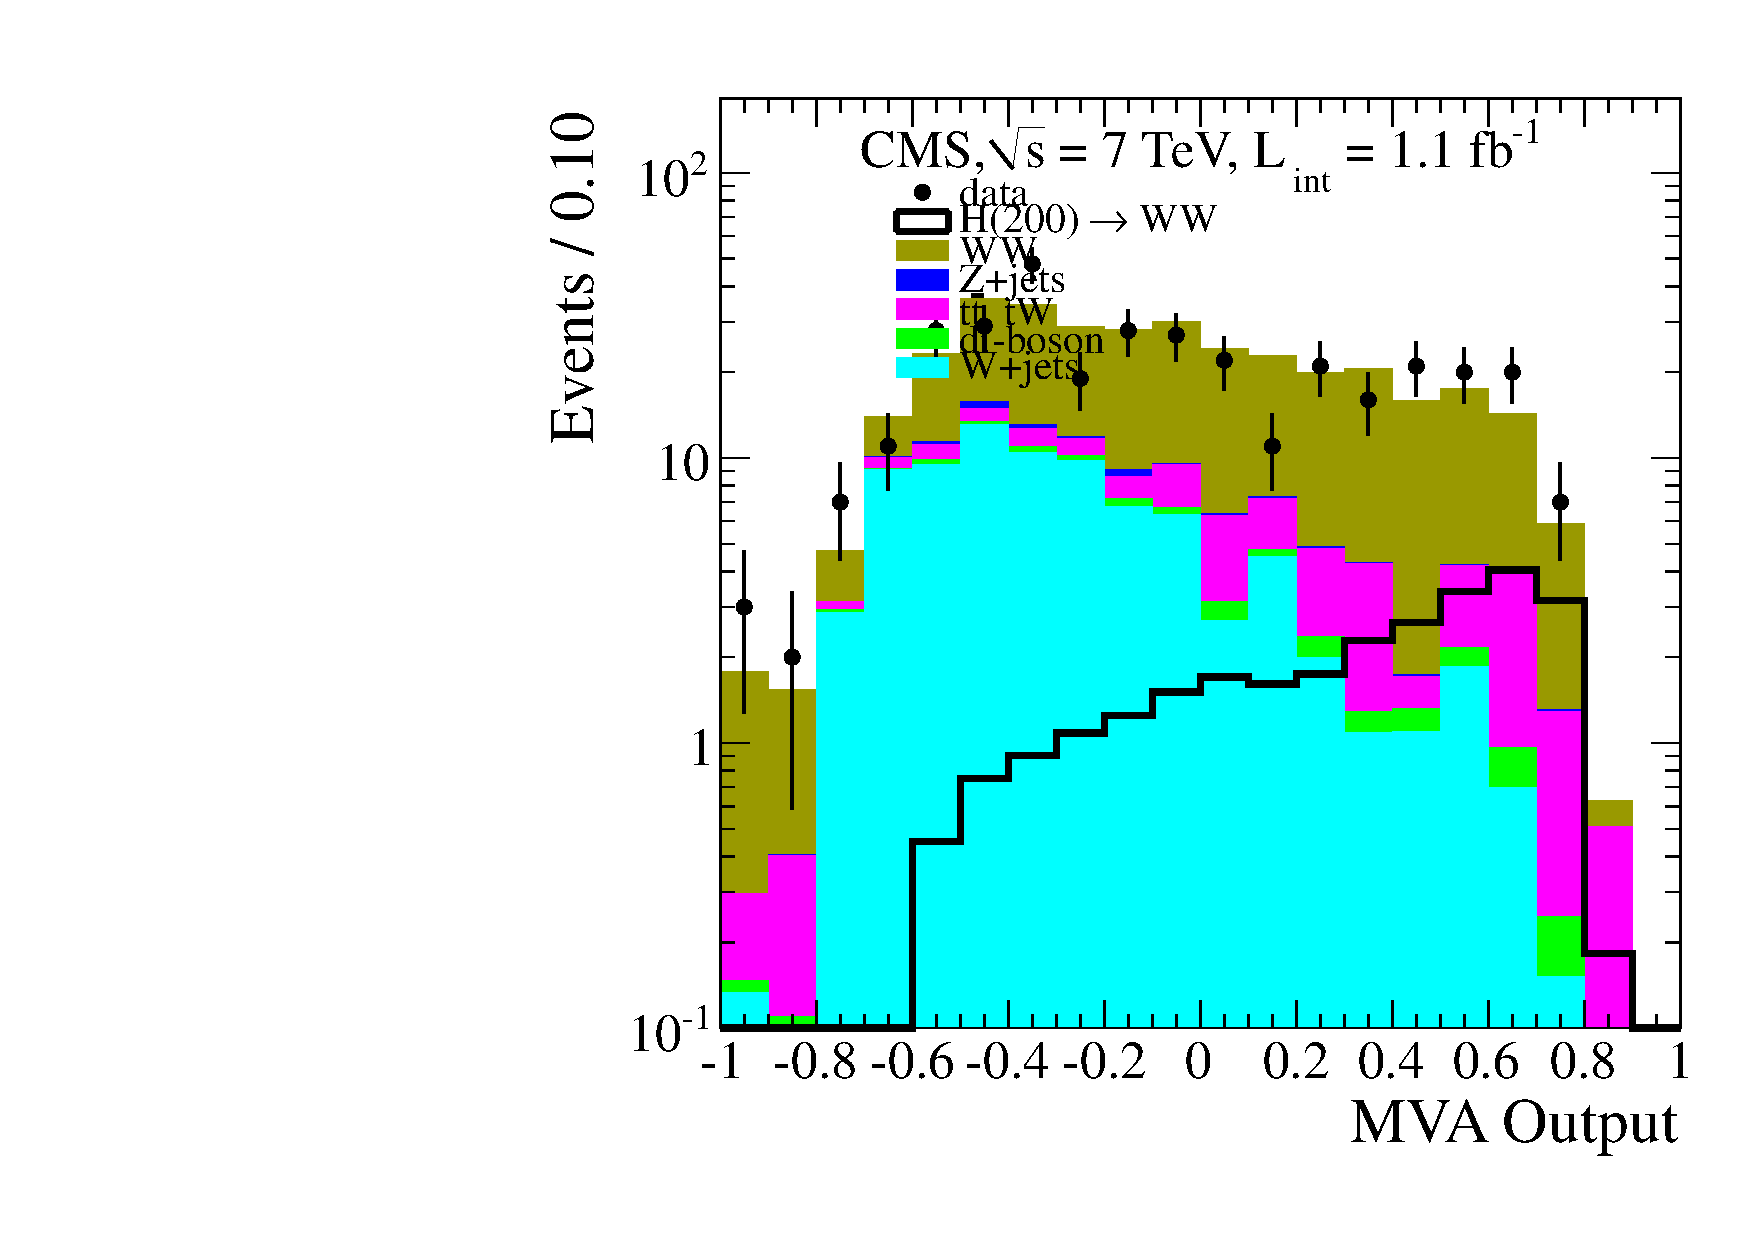
\includegraphics[width=0.49\textwidth,angle=0]{figures/histo_mva_200_0j_of.pdf}} 
   \subfigure[]{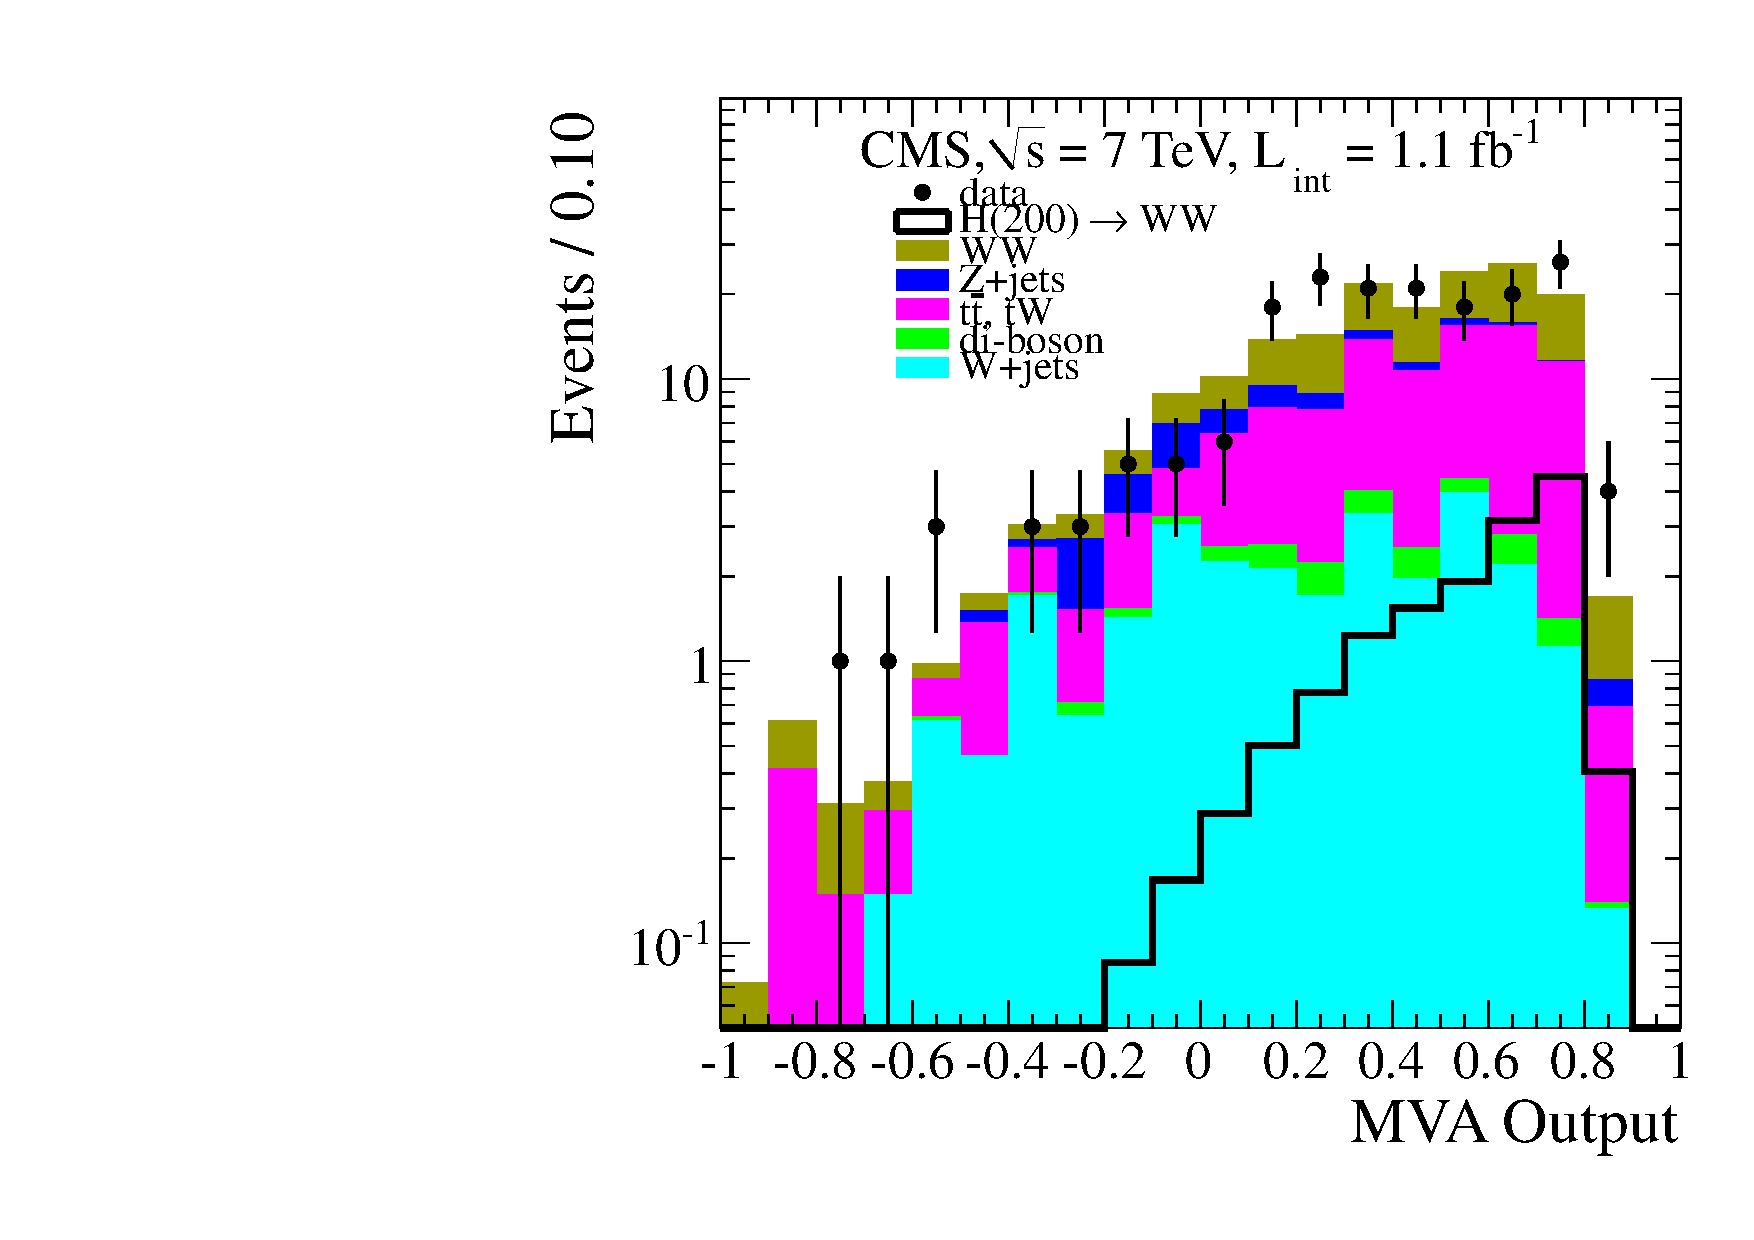
\includegraphics[width=0.49\textwidth,angle=0]{figures/histo_mva_200_1j_of.pdf}} 
       \caption{Classifier outputs for Higgs signal and background events 
for \mHi=200 $\GeVcc$ in the 0-jet bin same flavor final state (a), 1-jet bin same flavor final state (b), 
 0-jet bin opposite flavor final state (c), and 1-jet bin opposite flavor final state (d), after the $\WW$ selection. The number 
of events is different on each mass point due to the specific $\mll$ requirement.}
   \label{fig:histo_mva_200}
\end{center}
\end{figure}

\begin{table}[!ht]
  \begin{center}
 {\normalsize
  \begin{tabular} {|c|c|c|c|c|c|}
\hline
  mass    & SM $H\to WW$ & all bkg. & $qq \to \WW$ & $gg \to \WW$ & {\small $WZ$/$ZZ$ not included in the $\dyll$} \\
  \hline
  \hline
115 &    5.3 $\pm$ 0.1 &  52.5 $\pm$ 2.4  &  25.4 $\pm$ 0.4 &   1.1 $\pm$ 0.0 &   0.8 $\pm$ 0.1 \\
120 &    9.5 $\pm$ 0.1 &  61.8 $\pm$ 2.5  &  33.1 $\pm$ 0.5 &   1.4 $\pm$ 0.0 &   0.9 $\pm$ 0.1 \\
130 &   21.1 $\pm$ 0.2 &  75.6 $\pm$ 2.6  &  46.3 $\pm$ 0.6 &   2.3 $\pm$ 0.1 &   1.2 $\pm$ 0.1 \\
140 &   24.3 $\pm$ 0.3 &  48.9 $\pm$ 1.7  &  34.8 $\pm$ 0.5 &   2.0 $\pm$ 0.1 &   0.8 $\pm$ 0.1 \\
150 &   25.9 $\pm$ 0.3 &  28.9 $\pm$ 0.9  &  23.3 $\pm$ 0.4 &   1.8 $\pm$ 0.1 &   0.5 $\pm$ 0.1 \\
160 &   40.0 $\pm$ 0.4 &  23.1 $\pm$ 1.0  &  17.4 $\pm$ 0.3 &   1.8 $\pm$ 0.1 &   0.3 $\pm$ 0.1 \\
170 &   33.9 $\pm$ 0.4 &  20.4 $\pm$ 1.0  &  14.7 $\pm$ 0.3 &   1.9 $\pm$ 0.1 &   0.3 $\pm$ 0.1 \\
180 &   22.7 $\pm$ 0.3 &  20.3 $\pm$ 0.9  &  13.8 $\pm$ 0.3 &   2.1 $\pm$ 0.1 &   0.3 $\pm$ 0.1 \\
190 &   19.8 $\pm$ 0.2 &  33.2 $\pm$ 1.2  &  22.9 $\pm$ 0.4 &   3.1 $\pm$ 0.1 &   0.6 $\pm$ 0.1 \\
200 &   11.8 $\pm$ 0.2 &  25.0 $\pm$ 1.0  &  16.6 $\pm$ 0.3 &   2.5 $\pm$ 0.1 &   0.5 $\pm$ 0.1 \\
250 &    5.9 $\pm$ 0.1 &  23.6 $\pm$ 1.1  &  15.4 $\pm$ 0.3 &   1.6 $\pm$ 0.0 &   0.4 $\pm$ 0.1 \\
300 &    5.9 $\pm$ 0.1 &  29.2 $\pm$ 1.3  &  19.2 $\pm$ 0.4 &   1.5 $\pm$ 0.0 &   0.4 $\pm$ 0.1 \\
350 &    5.9 $\pm$ 0.1 &  24.0 $\pm$ 1.1  &  15.3 $\pm$ 0.3 &   1.1 $\pm$ 0.0 &   0.4 $\pm$ 0.1 \\
400 &    4.9 $\pm$ 0.1 &  22.2 $\pm$ 1.1  &  13.5 $\pm$ 0.3 &   0.9 $\pm$ 0.0 &   0.3 $\pm$ 0.1 \\
450 &    3.0 $\pm$ 0.0 &  16.3 $\pm$ 1.0  &   9.6 $\pm$ 0.3 &   0.7 $\pm$ 0.0 &   0.3 $\pm$ 0.1 \\
500 &    1.7 $\pm$ 0.0 &  12.2 $\pm$ 0.8  &   6.7 $\pm$ 0.2 &   0.6 $\pm$ 0.0 &   0.2 $\pm$ 0.0 \\
550 &    1.1 $\pm$ 0.0 &  11.2 $\pm$ 0.8  &   6.3 $\pm$ 0.2 &   0.5 $\pm$ 0.0 &   0.2 $\pm$ 0.0 \\
600 &    0.6 $\pm$ 0.0 &   7.3 $\pm$ 0.6  &   4.0 $\pm$ 0.2 &   0.3 $\pm$ 0.0 &   0.1 $\pm$ 0.0 \\
 \hline
  \end{tabular}
  }
 {\normalsize
  \begin{tabular} {|c|c|c|c|}
\hline
  mass    & $\ttbar+tW$ & $\dyll+WZ+ZZ$ & $\Wjets$ \\
  \hline
  \hline
115 &  1.9 $\pm$ 0.4 &   1.9 $\pm$ 0.4 &  16.5 $\pm$ 2.1 \\
120 &  2.2 $\pm$ 0.5 &   1.9 $\pm$ 0.4 &  17.9 $\pm$ 2.3 \\
130 &  2.6 $\pm$ 0.5 &   2.2 $\pm$ 0.4 &  17.6 $\pm$ 2.3 \\
140 &  2.3 $\pm$ 0.5 &   1.2 $\pm$ 0.2 &   6.8 $\pm$ 1.5 \\
150 &  1.1 $\pm$ 0.3 &   0.8 $\pm$ 0.2 &   1.3 $\pm$ 0.8 \\
160 &  1.2 $\pm$ 0.3 &   0.7 $\pm$ 0.2 &   1.8 $\pm$ 0.9 \\
170 &  1.7 $\pm$ 0.4 &   0.6 $\pm$ 0.2 &   1.2 $\pm$ 0.8 \\
180 &  2.3 $\pm$ 0.5 &   0.6 $\pm$ 0.2 &   1.2 $\pm$ 0.7 \\
190 &  3.7 $\pm$ 0.6 &   0.7 $\pm$ 0.1 &   2.1 $\pm$ 0.9 \\
200 &  3.5 $\pm$ 0.6 &   0.7 $\pm$ 0.1 &   1.2 $\pm$ 0.7 \\
250 &  4.6 $\pm$ 0.7 &   0.6 $\pm$ 0.1 &   0.8 $\pm$ 0.7 \\
300 &  5.3 $\pm$ 0.7 &   0.5 $\pm$ 0.0 &   2.2 $\pm$ 0.9 \\
350 &  4.9 $\pm$ 0.7 &   0.4 $\pm$ 0.0 &   1.8 $\pm$ 0.7 \\
400 &  4.7 $\pm$ 0.7 &   0.3 $\pm$ 0.0 &   2.4 $\pm$ 0.8 \\
450 &  3.5 $\pm$ 0.6 &   0.2 $\pm$ 0.0 &   2.0 $\pm$ 0.7 \\
500 &  3.1 $\pm$ 0.6 &   0.1 $\pm$ 0.0 &   1.6 $\pm$ 0.5 \\
550 &  2.8 $\pm$ 0.6 &   0.1 $\pm$ 0.0 &   1.3 $\pm$ 0.5 \\
600 &  1.6 $\pm$ 0.4 &   0.1 $\pm$ 0.0 &   1.1 $\pm$ 0.4 \\
 \hline
  \end{tabular}
  }
  \caption{Expected number of signal and background processes for an 
  integrated luminosity of $\intlumi$, after applying the full multivariate analysis 
  selection in the 0-jet bin case. Monte Carlo statistical uncertainties are included.}
   \label{tab:mvasel0j}
  \end{center}
\end{table}

\begin{table}[!ht]
  \begin{center}
 {\normalsize
  \begin{tabular} {|c|c|c|c|c|c|}
\hline
  mass    & SM $H\to WW$ & all bkg. & $qq \to \WW$ & $gg \to \WW$ & {\small $WZ$/$ZZ$  not included in the $\dyll$} \\
  \hline
  \hline
115 &   1.6 $\pm$ 0.0 &  18.6 $\pm$ 1.4  &   6.3 $\pm$ 0.2 &   0.3 $\pm$ 0.0 &   0.6 $\pm$ 0.1 \\
120 &   3.3 $\pm$ 0.1 &  24.9 $\pm$ 1.6  &   8.4 $\pm$ 0.2 &   0.4 $\pm$ 0.0 &   0.8 $\pm$ 0.1 \\
130 &   6.4 $\pm$ 0.1 &  25.1 $\pm$ 1.6  &   8.9 $\pm$ 0.2 &   0.5 $\pm$ 0.0 &   0.7 $\pm$ 0.1 \\
140 &   9.5 $\pm$ 0.1 &  21.9 $\pm$ 1.4  &   9.2 $\pm$ 0.2 &   0.6 $\pm$ 0.0 &   0.5 $\pm$ 0.1 \\
150 &  10.6 $\pm$ 0.2 &  16.4 $\pm$ 1.1  &   7.1 $\pm$ 0.2 &   0.5 $\pm$ 0.0 &   0.4 $\pm$ 0.1 \\
160 &  18.8 $\pm$ 0.2 &  15.0 $\pm$ 0.9  &   7.1 $\pm$ 0.2 &   0.6 $\pm$ 0.0 &   0.3 $\pm$ 0.1 \\
170 &  15.5 $\pm$ 0.2 &  12.4 $\pm$ 0.7  &   6.9 $\pm$ 0.2 &   0.6 $\pm$ 0.0 &   0.2 $\pm$ 0.0 \\
180 &  10.1 $\pm$ 0.2 &  13.3 $\pm$ 0.9  &   6.5 $\pm$ 0.2 &   0.6 $\pm$ 0.0 &   0.2 $\pm$ 0.0 \\
190 &  10.5 $\pm$ 0.1 &  24.4 $\pm$ 1.3  &  12.0 $\pm$ 0.3 &   1.1 $\pm$ 0.0 &   0.4 $\pm$ 0.1 \\
200 &   6.4 $\pm$ 0.1 &  20.9 $\pm$ 1.1  &  10.7 $\pm$ 0.3 &   1.0 $\pm$ 0.0 &   0.2 $\pm$ 0.0 \\
250 &   3.9 $\pm$ 0.1 &  26.9 $\pm$ 1.5  &  11.1 $\pm$ 0.3 &   0.5 $\pm$ 0.0 &   0.4 $\pm$ 0.1 \\
300 &   3.3 $\pm$ 0.0 &  21.2 $\pm$ 1.4  &   8.4 $\pm$ 0.2 &   0.4 $\pm$ 0.0 &   0.3 $\pm$ 0.1 \\
350 &   4.6 $\pm$ 0.1 &  27.4 $\pm$ 1.4  &  10.5 $\pm$ 0.3 &   0.6 $\pm$ 0.0 &   0.5 $\pm$ 0.1 \\
400 &   4.0 $\pm$ 0.0 &  23.2 $\pm$ 1.4  &   8.7 $\pm$ 0.2 &   0.5 $\pm$ 0.0 &   0.4 $\pm$ 0.1 \\
450 &   2.1 $\pm$ 0.0 &  14.1 $\pm$ 1.2  &   4.9 $\pm$ 0.2 &   0.3 $\pm$ 0.0 &   0.2 $\pm$ 0.0 \\
500 &   1.4 $\pm$ 0.0 &  11.1 $\pm$ 1.0  &   3.9 $\pm$ 0.2 &   0.2 $\pm$ 0.0 &   0.1 $\pm$ 0.0 \\
550 &   0.9 $\pm$ 0.0 &   9.3 $\pm$ 0.9  &   3.3 $\pm$ 0.1 &   0.2 $\pm$ 0.0 &   0.1 $\pm$ 0.0 \\
600 &   0.6 $\pm$ 0.0 &   6.7 $\pm$ 0.8  &   2.2 $\pm$ 0.1 &   0.1 $\pm$ 0.0 &   0.1 $\pm$ 0.0 \\
 \hline
  \end{tabular}
  }
 {\normalsize
  \begin{tabular} {|c|c|c|c|}
\hline
  mass    & $\ttbar+tW$ & $\dyll+WZ+ZZ$ & $\Wjets$  \\
  \hline
  \hline
115 &   4.6 $\pm$ 0.7 &   1.9 $\pm$ 0.4 &  3.9 $\pm$ 1.1 \\
120 &   5.5 $\pm$ 0.8 &   4.3 $\pm$ 0.6 &  4.4 $\pm$ 1.2 \\
130 &   6.4 $\pm$ 0.9 &   4.2 $\pm$ 0.6 &  3.4 $\pm$ 1.0 \\
140 &   6.7 $\pm$ 0.9 &   1.5 $\pm$ 0.3 &  2.9 $\pm$ 1.0 \\
150 &   5.4 $\pm$ 0.8 &   0.9 $\pm$ 0.3 &  1.6 $\pm$ 0.6 \\
160 &   5.2 $\pm$ 0.7 &   0.8 $\pm$ 0.2 &  0.5 $\pm$ 0.4 \\
170 &   4.0 $\pm$ 0.6 &   0.7 $\pm$ 0.2 &  0.0 $\pm$ 0.0 \\
180 &   4.9 $\pm$ 0.7 &   0.6 $\pm$ 0.2 &  0.3 $\pm$ 0.3 \\
190 &   8.7 $\pm$ 1.0 &   0.9 $\pm$ 0.3 &  1.2 $\pm$ 0.7 \\
200 &   7.3 $\pm$ 0.9 &   0.9 $\pm$ 0.3 &  0.7 $\pm$ 0.6 \\
250 &  12.6 $\pm$ 1.2 &   0.6 $\pm$ 0.2 &  1.7 $\pm$ 0.8 \\
300 &  11.1 $\pm$ 1.2 &   0.3 $\pm$ 0.1 &  0.6 $\pm$ 0.6 \\
350 &  15.5 $\pm$ 1.4 &   0.4 $\pm$ 0.1 &  0.0 $\pm$ 0.0 \\
400 &  13.5 $\pm$ 1.3 &   0.1 $\pm$ 0.0 &  0.0 $\pm$ 0.5 \\
450 &   8.2 $\pm$ 1.0 &   0.1 $\pm$ 0.0 &  0.4 $\pm$ 0.5 \\
500 &   6.1 $\pm$ 0.9 &   0.0 $\pm$ 0.0 &  0.7 $\pm$ 0.5 \\
550 &   5.3 $\pm$ 0.8 &   0.1 $\pm$ 0.0 &  0.4 $\pm$ 0.4 \\
600 &   3.9 $\pm$ 0.7 &   0.0 $\pm$ 0.0 &  0.4 $\pm$ 0.4 \\
 \hline
  \end{tabular}
  }
  \caption{Expected number of signal and background processes for an 
  integrated luminosity of $\intlumi$, after applying the full multivariate analysis 
  selection in the 1-jet bin case. Monte Carlo statistical uncertainties are included.}
   \label{tab:mvasel1j}
  \end{center}
\end{table}
